% se puede agregar la opción [english] para 
%  memorias o tesis en inglés (borrando el archivo .aux)
\documentclass{umemoria} 

\depto{Departamento de Física}
\author{Benjamín Ignacio Pérez Estay}
\title{Characterization of \textit{E.coli} swimming near sinusoidal surfaces }

% incluir ambos comandos para una doble titulación
%  o quitar el comando que no aplica
\tesis{Magíster en Ciencias, mención Física}
%\tesis{Doctor en ???} % incluir solo este comando para doctorados

% puede haber varios profesores guía seperados por coma;
% pero si es una memoria, solo puede haber un profesor guía
\guia{Rodrigo Soto, María Luisa Cordero, Néstor Sepúlveda} 

% puede haber varios profesores co-guía seperados por coma;
% pero si es una memoria, el profesor co-guía será el primer
% integrante de la comisión
%\coguia{Nombre Completo Co-Guía} % incluir en caso de co-guía de *tesis*

%\cotutela{Nombre Institución} % incluir en caso de cotutela

\comision{Nombre Completo Uno,Nombre Completo Dos,Nombre Completo Tres}

%\auspicio{Nombre Institución} % incluir en caso de recibir financiamiento

% tiene que ser el año en que se da el examen de título/grado (defensa)
%\anho{2021} % incluir solo para reemplazar el año actual

\usepackage{lipsum}
\usepackage{xcolor}
\usepackage{svg}
\usepackage{float}
\usepackage{wrapfig, blindtext}
\usepackage{siunitx}
\usepackage{makecell}
\usepackage{tabularx}
\usepackage{afterpage}
\usepackage{fancyhdr}
\usepackage{changepage}
\DeclareSIUnit\rpm{rpm}
\DeclareSIUnit\molar{M}
\DeclareSIUnit\OD{OD$_{600}$}
\DeclareSIUnit\cells{cells}
\DeclareSIUnit\pixels{px}
\bibliographystyle{ieeetr}

\setlength{\parindent}{0pt}

\begin{document}

\frontmatter
\maketitle

\begin{adjustwidth}{4.2cm}{}
\begin{tabular}{l}
	\MakeUppercase{abstract of the thesis for the degree } \\
	\MakeUppercase{of master of science, mention in physics}\\
	BY: BENJAMÍN PÉREZ \\
	DATE: \MakeUppercase{\today} \\
	SUPERVISORS: MARÍA LUISA CORDERO, NÉSTOR SEPÚLVEDA, \\ 
    RODRIGO SOTO\\
\end{tabular}
\end{adjustwidth}

\begin{center}
    \MakeUppercase{Characterization of \textit{E.coli} swimming near sinusoidal surfaces }
\end{center}

Bacteria swim thanks to the movement of their flagella. That affirmation branches in many forms, as bacteria have different body shapes and flagella types. Moreover, the environment plays a crucial role. Swimming in the ocean with flows or near a surface is not the same. Flat surfaces have been found to trap bacteria, eventually resulting in their adhesion to the surface and the initiation of biofilm formation. Avoiding biofilm formation is an open medical problem whose solution would save lives. This thesis studies, both experimentally and theoretically, how surface shape can modify cell trapping. The main idea is that a microscopic sinusoidal wall could reorient cells and expel them away from the wall. 

The first chapter explains the main concepts required to understand this work and its relevance. The second chapter describes the protocols for bacteria culture, fabrication of the microfluidic devices, data acquisition, and analysis. Experiments were performed with a genetically modified strain of \textit{E.coli} that does not tumble because it is less likely for them to leave the surface. Also, bacterial density was kept low to observe individual bacteria movement. 

The third chapter presents a theoretical framework for the numerical description of the bacterial dynamics with minimal components. This leads us to an agent-based model of spherical active Brownian particles in a two-dimensional representation that considers elastic collisions and steric alignments with the wall.

Chapter 4 shows the results obtained in the experiments and the model, which show that the curvature of the sinusoidal wall plays a fundamental role. When the curved wall is almost flat, the bacteria hardly come out of the wall. On the other hand, if the valleys are too narrow, bacteria will be trapped there. Varying the amplitude and wavelength of the surface profile, a transition between these two regimes is found. The critical regime represents the case where bacteria can still move through the valley quickly, but the escape angle is higher, causing the bacteria to leave the surface, leading to a minimum in the accumulation. Measured velocities in the tracking of bacteria support this result. The numerical model qualitatively reproduces experimental observations adjusting only two parameters, the rotational diffusion coefficient and the magnitude of the alignment interaction with the wall. This simplicity allows us to conclude that the alignment of the cells with the wall is the cause of this phenomenon, while other effects caused by hydrodynamic interactions with the wall and between cells are negligible. Because many bacteria experience steric forces in a similar way, this study promises to apply to other bacterial species. 

Finally, chapter 5 summarizes the conclusions and perspectives of this work. 


\newpage
\begin{adjustwidth}{4.2cm}{}
\begin{tabular}{l}
	RESUMEN DE LA MEMORIA PARA OPTAR AL GRADO\\
	DE MAGÍSTER EN CIENCIAS, MENCIÓN FÍSICA \\
	POR: BENJAMÍN PÉREZ \\
	FECHA: \MakeUppercase{\today} \\
	PROF. GUÍA: RODRIGO SOTO, MARÍA LUISA CORDERO, \\
	NÉSTOR SEPÚLVEDA\\
\end{tabular}
\end{adjustwidth}

\begin{center}
    \MakeUppercase{Caracterización del nado de \textit{E.coli} cerca de paredes sinusoidales }
\end{center}

Las bacterias nadan gracias al movimiento de sus flagelos. Esa afirmación se ramifica de muchas maneras, ya que las bacterias tienen diferentes formas corporales y tipos de flagelos. Además, el entorno tiene un papel crucial. No es lo mismo nadar en el océano con flujos o cerca de una superficie. Se ha visto que las superficies planas atrapan a las bacterias, eventualmente provocando su adhesión a la superficie y el inicio de la formación de biofilms. Evitar la formación de biofilm es un problema abierto cuya solución salvaría vidas. En esta tesis se estudiará experimental y teóricamente, cómo la forma de la superficie puede modificar el atrapamiento de las celulas. La idea principal es que una pared microscópica sinusoidal podría reorientar las células, expulsandolas lejos de la pared. 

El primer capítulo, explica los conceptos principales requeridos para entender este trabajo y su relevancia. El segundo capítulo describe los protocolos de cultivo de bacterias, la fabricación de los dispositivos microfluídicos, las mediciones y su análisis. Los experimentos se hicieron con una cepa modificada genéticamente de \textit{E.coli} que no hace giros porque eso supone una menor probabilidad de abandonar una superficie. La densidad se mantuvo baja, para poder observar el movimiento de bacterias individuales.

El tercer capítulo presenta un marco teórico que describe como simular numéricamente la dinámica de las bacterias con ingredientes mínimos. Esto nos lleva a un modelo microscópico de partículas brownianas activas esféricas en una representación bidimensional que considera colisiones elásticas y alineamientos estéricos con la pared.

El capítulo 4 muestra los resultados obtenidos en los experimentos y el modelo, que demuestran que la curvatura de la pared sinusoidal juega un papel fundamental. Cuando la pared curva es casi plana, las bacterias apenas salen de la pared. Por otro lado, si el valle es demasiado estrecho, las bacterias quedarán atrapadas ahí. Variando la amplitud y la longitud de onda del perfil de la superficie, se encuentra una transición entre estos dos regímenes. El punto crítico representa el caso en que las bacterias aún pueden moverse por el valle, pero el ángulo de escape es mayor provocando que las bacterias salgan de la superficie, causando un mínimo en la acumulación. Mediciones de la velocidad vía tracking apoyan este resultado. El modelo numérico reproduce cualitativamente las observaciones experimentales ajustando solo dos parámetros, el coeficiente de difusión rotacional y la magnitud del alineamiento con la pared. Esta simplicidad permite concluir que el alineamiento de las células con la pared es la causa de este fenómeno, mientras que otros efectos causados por interacciones hidrodinámicas son despreciables. Debido a que muchas bacterias experimentan fuerzas estéricas con la pared de forma similar, este estudio promete aplicar a otras especies de bacterias.

El capítulo 5 resume las conclusiones y perspectivas de este trabajo.



\begin{dedicatoria}
Una dedicatoria corta.
\end{dedicatoria}

\begin{thanks}
\lipsum[1-2]
\end{thanks}

\tableofcontents
\listoftables % opcional
\listoffigures % opcional

\mainmatter

\chapter{Introduction}

Life is a beautiful phenomenon. We struggle to find it in other parts of the universe, yet in our planet is everywhere. Even in the most inhospitable places, such as volcanoes and deserts, life flourishes. Also, life comes in different forms as living organisms are roughly classified into five very different kingdoms. Such diversity raises many questions for scientists interested in understanding life. Biophysicists are devoted to revealing the intricacies of living organisms via physics and sometimes chemistry. This novel approach has gained much attention, as physics provides a fundamental vision of the phenomena that allow us to understand them in a broader sense, grouping those with a common interpretation.

Biophysics has addressed topics of various parts of life. There are studies with a physical approach on cell membranes \cite{Nguyen2021PhotocatalyticSynthesis,Jin2020MechanosensitiveMechanisms,Janmey2006BiophysicalMembranes}, biological macromolecules \cite{Allewell2013MolecularSciences, 2008MethodsFunction, Fierz2019BiophysicsDynamics}, evolution \cite{Sikosek2014BiophysicsBiophysics}, bacteria movement \cite{Lauga2020TheMotility, Ananthakrishnan2007TheMovement}, diseases such as cancer and Alzheimer's \cite{White2019TheCancer, Weickenmeier2019ASclerosis} and much else. Physics has already brought to these topics fundamental explanations, which contributed to typically descriptive biology in the quest to understand life. Biophysics has proven its usefulness in a few decades.

This thesis focuses on studying the interaction between bacteria and sinusoidal walls from a biophysical point of view to control or reduce biofilm formation.

\section{Biofilm}

Biofilms are consortiums of cells living on a surface. These cells secrete polymers, typically proteins and polysaccharides, which form an extracellular matrix that the cells share. Mechanisms employed in biofilm formation vary depending on strains and environmental conditions. Biofilm is a structure challenging to deal with, as antibiotics have proven to fail at killing bacteria in biofilm even at a concentration 1000 times higher than the normal concentration that kills floating bacteria \cite{Costerton1987BacterialDisease.}. This means that biofilm is a chronic bacterial infection.

\afterpage{%
\begin{figure}[H]
	\centering
	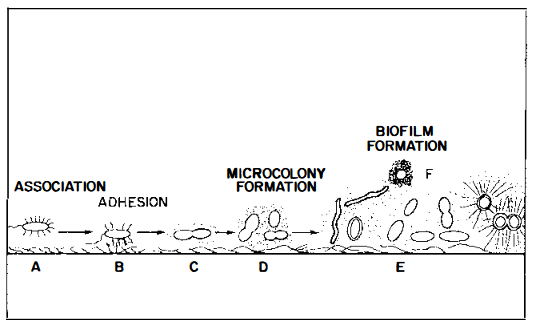
\includegraphics[width=\linewidth]{imagenes/BiofilmFormation.PNG}
	\caption[Diagram of biofilm formation]{ Diagram of biofilm formation in chronological order. a) Reversible association of a bacteria with a surface. b) Irreversible adhesion of bacteria, due to chemical or physical reasons. c) Cellular division leads to formation of microcolonies and aftwerwards d) biofilm structure is complete. (from \cite{Costerton1987BacterialDisease.})}
	\label{biofilm}
\end{figure}
}

Biofilm was not a problem in the early development of health care because it is relatively rare to have this kind of infection inside the human body. Due to this, biofilm was the last of the problems, but this has changed recently. This change relies on the cause of biofilm formation in the human body. ``The inability of the host and of therapeutic efforts to resolve acute infection triggers a series of events that culminates in a chronic condition" \cite{CiernyIII2006TreatmentInfection}. Diabetes and intra-corporal devices are contemporary reasons that decrease the ability of the body to resolve an infection, so biofilm appears. Badly treated diabetes can produce chronic hyperglycemia, associated with failure of blood vessels among many other organs \cite{2014DiagnosisMellitus}. This reduces wound healing as less blood reaches the wound; therefore, people with diabetes are an at-risk group for biofilm formation.

On the other hand, intra-corporal devices are made to replace something on a human body, compensating for the missing function. The problem is that intra-corporal devices are like dead tissue for the immune system. This means that any bacteria that attach to this surface will be harder to reach. These device-related infections have interrupted the development of complex medical devices that could replace organs like the heart. If these mechanical organs are susceptible to infections, they bring more problems than solutions \cite{Costerton1999IntroductionBiofilm}. Considering this, developing technology that prevents biofilm formation has brought interest as it could allow new medical technology.

\subsection{Objective: interrupt biofilm formation}

Biofilm formation begins with the association of a bacterium to a surface. This means that the bacteria are near or in contact with the surface. Bacteria are attracted to the surface due to hydrodynamic effects, and some species can even sense the presence of a surface by signaling molecules. This state of association is reversible as bacteria are still moving on the surface. Depending on the species, bacteria may move very little or explore the surface before adhering \cite{Costerton1999IntroductionBiofilm}. Once adhered, due to chemical or physical reasons, the process is irreversible. The cell will divide, forming microcolonies of bacteria whose secretions will form the extracellular matrix that composes the biofilm. Therefore, to reduce biofilm formation, it is essential to revert the association of bacteria with a surface before the adhesion takes place. To do so, the chemical and physical properties of the surface must be tweaked.

Considering the above, the objective of this thesis is to \textbf{generate a surface that makes bacteria move away from it due to its sinusoidal geometry}, thus preventing cell adhesion. This will be done experimentally in in vitro systems, i.e., in controlled non-living environments. In addition, \textbf{a model of the system will be generated to pursue a fundamental physical explanation of the experimental observations}. This complementation between experiments and simulations will allow a deeper understanding of the results. The rest of the chapter introduces the physical effects that led to this objective. In section \ref{section:active matter} we describe bacteria movement in general and later on focus on \textit{E. coli} the species we used in experiments. Meanwhile, section \ref{section:surface effects} describes the effects of surfaces in bacteria swimming and the idea behind using a sinusoidal surface.

\section{Active matter}
\label{section:active matter}

In this thesis, we focus on the interaction between \textit{E. coli} bacteria and a surface. The area of biophysics that encompasses this subject is known as active matter. Active matter studies complex systems with the perspective that the active motion of every particle is the key to understanding the phenomena. Active motion refers to the idea that a particle obtains energy from the medium to propel itself. This is a common feature of organisms such as prokaryotic cells and animals. Interactions between particles or their environment lead to fascinating phenomena. Flock of birds \cite{Bialek2012StatisticalBirds,Cavagna2015FlockingMotion}, schools of fish \cite{Toner1998FlocksFlocking}, bacterial suspensions \cite{Lopez2015TurningSuperfluids, Clement2016BacterialFlow,Vincenti2019MagnetotacticMotor}, crowds of people \cite{Faria2010LeadershipCrowds} and even artificially active colloidal particles \cite{Zhang2018Light-controlledParticles, Jiang2020PickeringApplications} are examples of active matter. Typically, these systems exhibit interesting collective behavior. For example, in flocks and schools, individuals move more or less in the same direction and are able to follow as a whole the change of direction proposed by leaders. This collective movement is a survival method that allows the flock to avoid attack by predators \cite{Bialek2012StatisticalBirds,Cavagna2015FlockingMotion}.


\afterpage{%
\begin{figure}[H]
	\centering
	\includesvg[width=\linewidth]{imagenes/activeMatter}
	\caption[Examples of active matter]{Examples of active matter. Flocks of birds, school of fish and crowds are examples of macroscopical active matter. Bacteria and active colloids on the other hand are microscopical examples. }
	\label{experimental profiles}
\end{figure}
}

\subsection{Bacterial suspensions}

Among these examples, we are interested in the culture of bacteria in fluids, called bacterial suspensions. Bacteria are grown in a rich medium but not necessarily observed in such conditions because by centrifugation, they can be transferred to scarcer media. Bacterial suspensions are put in microscopic environments to study the dynamics of the cells. This is attractive because the behavior of bacteria can be controlled by using different species or even by genetic modifications. Individuals of the same species \textit{E. coli} can move in straight lines instead of doing tumbles just by changing one gene \cite{VanVliet2014ThePopulations}. Genetic modifications produce new species strains that can better suit a specific study. Such possibilities make bacterial suspensions the playground of choice for active matter studies.

Bacteria have different mechanisms to move depending on their natural habitat. In solid surfaces, bacteria move through twitching, gliding, or usage of flagella. Flagella-driven movement is the most common type of movement, and it also allows swimming in liquids. Flagella structure has three parts, the basal body that produces rotation, the filament, a helical propeller, and the hook that connects both structures transmitting the torque from the body to the filament \cite{Nakamura2019Flagella-drivenBacteria}. Different species may have differently composed flagella and also a different number of flagella (see figure \ref{flagella}). 


\afterpage{%
\begin{figure}[H]
	\centering
	\includegraphics[width=\linewidth]{imagenes/flagella_full.png}
	\caption[Comparison of bacteria flagella of different species]{Electron micrographs of a) \textit{Salmonella} and b) \textit{E. coli} cells. Position and number of flagella are different. c) Structural differences in the basal body among bacterial species observed with electron cryotomography.  (adapted from \cite{Nakamura2019Flagella-drivenBacteria, Terashima2017StructuralSpecies}).  }
	\label{flagella}
\end{figure}
}



When swimming, the flagella of bacteria move coordinately to propel the body in one direction. This movement propels the bacteria with a force $\textbf{F}$. The body of the bacteria also experiments a drag force $-\textbf{F}$ due to the fluid resistance. Therefore, the effect of bacteria movement in fluids is modeled as a force dipole. This description has one degree of freedom called polarity. Polarity reveals whether the bacteria push or pull the fluid. Pushers have their flagella at the rear while the pullers have them at the front. An alternative description is that the pushers produce a flow away from their bodies, while pullers produce the opposite. In figure \ref{swimming methods} d) it is possible to see a comparison between the flow produced by these two swimming mechanisms. Flow-induced by bacteria produce hydrodynamic interactions between cells and also with surfaces. Such interactions have been extensively studied, and the effects of interest to us will be discussed in the following section. 

\afterpage{%
\begin{figure}[H]
	\centering
	\includesvg[width=\linewidth]{imagenes/swimming_methods}
	\caption[Force dipole approximation for bacteria swimming effects in fluids.]{a) Experimentally measured average flow flied produced by single \textit{E. coli}. b) Best-fit force dipole flow and c) the subtraction of the best-fit flow and the measured field. Parameters for the fitting include the magnitude of the forces $|\textbf{F}| =$ \SI{0.42}{\pico\newton} and the separation $\mathscr{l} =$ \SI{1.9}{\micro\meter} between the two forces (taken from \cite{Drescher2011FluidScattering}). d) Comparison between flows produced by spherical pushers and pullers in numerical simulations when moving upwards (taken from \cite{Zhu2012Self-propulsionPullers}).}
	\label{swimming methods}
\end{figure}
}

\subsection{\textit{Escherichia coli}}

In our study, we use the species of bacteria \textit{E. coli} because it is the most studied bacterial species. For example, as seen in figure \ref{swimming methods}, it has been proven that the first-order approximation of the dipole force scheme fits properly the flow produced by  \textit{E. coli} swimming at long ranges\cite{Drescher2011FluidScattering}. Near-field effects are not captured accordingly. Also, physical properties of \textit{E. coli} have been measured. Cells are rod-shaped and are about \SI{2}{\micro\meter} long and \SIrange[range-units=single]{0.5}{1}{\micro\meter} in diameter \cite{BritannicaOnlineEncyclopedia2021EducationEncyclopedia}. \textit{E. coli} produces around $5$ to $10$ flagella randomly distributed across the cell surface. When moving in straight lines or in a ``run", these flagella form a bundle that rotates in a counter-clockwise direction (when seen from behind). If any flagella start rotating clockwise, the bundle disassembles, and bacteria changes the direction of motion or ``tumbles". This movement is described as a run-and-tumble motion. The basal body of \textit{E. coli} rotates at \SI{10}{\hertz} and the typical tumble duration is \SI{0.1}{\second} \cite{Berg2001E.ColiMotion}. We measured the average speed of an \textit{E. coli} culture to be around \SIrange[range-units=single, per-mode = symbol]{18}{25}{\micro\meter \per \second}. The average speed depends on culture conditions such as temperature, oxygen presence, and manipulation. 

The specie \textit{E. coli} also has many mutant variations. It has been proven that up to $80\%$ of the genes in a typical genome of \textit{E. coli} are variable or ``accessory" genes \cite{Lukjancenko2010ComparisonGenomes}. In laboratories, \textit{E. coli} strains normally have a gene for expressing green (GFP) or red (mCherry) fluorescent proteins, allowing observation of bacteria only. For active matter studies, in particular, the most common genetic modification corresponds to the elimination of the synthesis of the cheY protein. This protein is involved in the transmission of sensory signals from the chemoreceptors to the flagellar motors, or in other words, regulates the chemotaxis in the cell. Therefore, cheY deletion causes the cell to stop tumbling. This is useful for studying particular properties of the swim that are independent of the tumbles or to avoid effects produced by tumbling and. We use this type of genetic modification in our experiments. Another typical example of genetic modifications is \textit{E. coli} strains rendered non-motile via deletion of motility proteins and then restored motility via inducible expression of the deleted gene from a plasmid. Other bacteria or a specific signal can regulate the induction. These strains lead to interesting dynamics, such as pattern formation and directed movement \cite{Ravichandar2017TranscriptionalGradient, Curatolo2020CooperativeRegulation}.

\section{Surface effects}
\label{section:surface effects}

\afterpage{%
\begin{figure}[H]
	\centering
	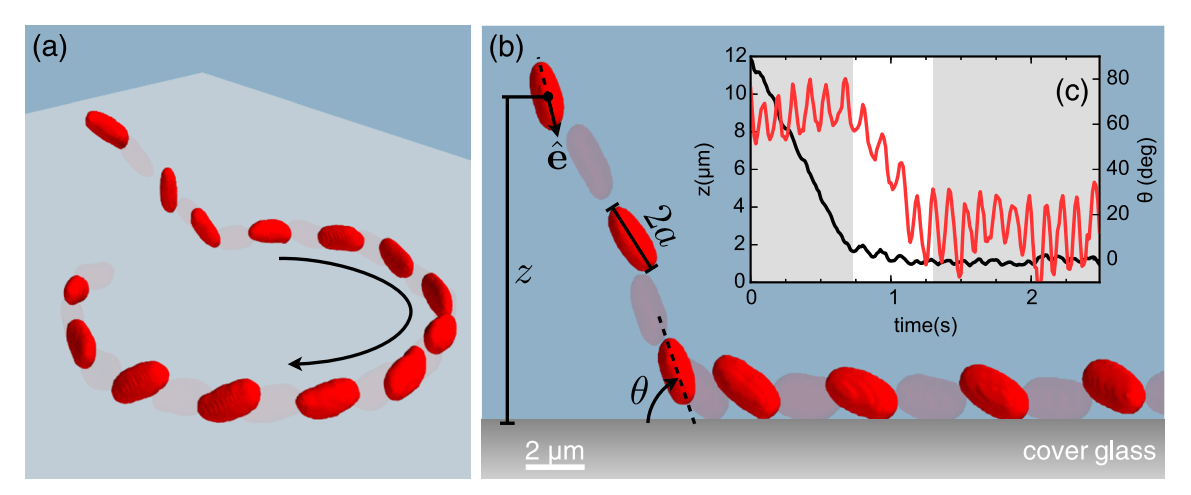
\includegraphics[width=\linewidth]{imagenes/3d_tracking.PNG}
	\caption[Volumetric reconstruction of bacteria during a wall-entrapment event.]{a) A sequence of volumetric reconstructions of swimming cells during a wall-entrapment event. b) A close and lateral view of another cell colliding with the wall. Time intervals between reconstructions are 0.2 s in both figures. (c) For the same cell as in (b), the wall distance is plotted as a black line, while the red line plots the angle of the cell-body axis. In both curves, three stages can be identified: approach to the wall, reorientation, and surface swimming. The grey shaded areas help to visualize these three stages. Taken from \cite{Bianchi2017HolographicBacteria}. }
	\label{3d_tracking}
\end{figure}
}


When \textit{E. coli} bacteria approach a surface, several physical effects affect their dynamics. These effects produce the association of the bacteria with the surface, causing the bacteria to remain swimming in contact with the surface. It should be emphasized that these effects occur prior to adhesion. We are interested in these effects because our objective is to prevent adhesion from occurring. Bianchi \textit{et al.} \cite{Bianchi2017HolographicBacteria} described these effects clearly by separating them into three stages. The wall approach stage, the steric reorientation stage, and the surface swimming stage.

First, in the wall approach stage, the cell is not in contact with the wall, meaning there is no direct interaction. It is reasonable to think that in this stage, the dynamics should not be the same as when the bacteria are far from the surface. This change is associated with hydrodynamic effects caused by the flow generated by the movement of bacteria. For flat surfaces, this cell-surface hydrodynamic interaction has been measured to slow down \textit{E. coli} bacteria by around $20\%$ of their bulk velocity and on average not rotate bacteria except for nearly parallel swimming \cite{Bianchi2017HolographicBacteria}. Such results are not predicted accurately by the force dipole approximation because near field effects are more relevant \cite{Drescher2011FluidScattering}. 

The moment bacteria contact the wall, a steric force arises. This repulsive force prevents the bacterium from passing through the wall. Therefore, its magnitude is equal to the component of the force exerted by the flagellum in the direction perpendicular to the wall. This force will have an associated torque that will produce a reorientation of the cell until parallel to the surface. Therefore, this stage is called the reorientation stage. Near-field hydrodynamic interactions are still present, but steric reorientation is dominant for cells incident on the surface at a considerable angle.

Then, in the surface swimming phase, bacteria are now almost parallel to the surface, and the dynamics are governed by both the contact and viscous forces. When swimming away from the surface, bacteria swim in straight lines, and the viscous forces are opposite to that direction. Also, rotation of the flagella produces a rotation of the cell body in the axis of movement. When near a surface, new viscous forces appear. First, as can be seen, when pushing a ball on the surface of a pool, translation produces a rotation of the ball in the perpendicular direction to the movement contained in the surface plane. Second, the helical bundle of the flagella also experiment a force due to variations of the local drag coefficient when near a surface. Both of these effects couple and produce bacteria to move in circular trajectories when in contact with a wall \cite{Lauga2006SwimmingBoundaries}. Figure \ref{3d_tracking} a) shows a circular trajectory measured by three-axis holographic microscopy.

A similar hydrodynamic model also shows that the equilibrium contact angle with a flat surface is not zero due to viscous forces. Such predictions were verified experimentally by measuring the average contact angle of cells swimming in contact with a surface, which on average was \ang{5} \cite{Sipos2015HydrodynamicWalls}. In figure \ref{3d_tracking} c) the red plot shows that the angle wobbles around a mean different from zero. This leads to the trapping of bacteria on the surface, increasing the residence time of bacteria to times much greater than the usual time of reorientation. For non-tumbling \textit{E. coli} the average residence time has been measured to be \SI{64}{\second} \cite{Drescher2011FluidScattering} and  \SI{21}{\second} for \textit{E. coli} that tumble \cite{Junot2021Run-to-tumbleBacteria}. This cell trapping is responsible for the accumulation of bacteria on a flat surface.

Another species of bacteria may experience other physical effects. For example, for puller swimmers, since the flagella are at the front of the body, direct contact between the flagella and the surface dominates the dynamic. Instead of an alignment, such interactions produce a surface scattering of the cells. This has been observed for the eukaryotic \textit{Chlamydomonas} algae \cite{Kantsler2013CiliaryEukaryotes}. 

There are also differences between in vitro and in vivo environments. In vitro systems have considerably different conditions from natural ones, where surfaces are coated with adsorbed polymers. Cell adhesion is more likely in such surfaces as the polymers may block cell movement. Moreover, in experiments, bacteria are grown in rich media, while in reality, bacteria live deprived of some minerals or nutrients. Cell membranes are susceptible to such changes in the growth medium. In in vivo situations, the cell membrane develops structures to adapt to environmental conditions, which alters the adhesion process \cite{Brown1985TheInfections.}. This means there are biological effects since bacteria can sense the presence of a surface and react to its presence \cite{Kimkes2019HowContact,Laventie2020SurfaceBacteria}. This should be kept in mind because we cannot fully generalize the results of this study. Even so, the complexity of in vivo systems, in the sense of their irreproducibility and inhomogeneity, means that in vitro studies are still relevant. Moreover, even though several studies have been done in in vitro environments, there are still aspects of the interplay between surface geometry and cell accumulation that are not understood.

\subsection{Curved surfaces}

\afterpage{%
\begin{figure}[H]
	\centering
	\includesvg[width=\linewidth]{imagenes/curved_surfaces}
	\caption[Curved surfaces studied in the literature]{Example of curved surfaces studied in the literature. a) Microscopical wells of nanometric depth distributed in different patterns. Each pattern has its own profile below the image and the colors indicate depth (taken from \cite{Perera-Costa2014StudyingPatterns}. b) Sharklet$^{TM}$ surface that biommimcs the skin of sharks shown in c), reducing biofouling (taken from \cite{Reddy2011MicropatternedColi}).} 
	\label{experimental profiles}
\end{figure}
}

A scientific community has focused on physical rather than chemical alternatives to interrupt biofilm formation because bacteria evolve rapidly and become resistant to such substances. As a result, several studies have focused on using surface topography to prevent colony formation. Many topography designed surfaces have helped decrease bacteria accumulation, such as microscopic wells of nanometric depth homogeneously distributed in space s \cite{Perera-Costa2014StudyingPatterns}, diamond-like patterns inspired in sharkskin \cite{Reddy2011MicropatternedColi} and hierarchically wrinkled surface topographies having wrinkles of different length scales (generations) ranging from tens of nanometers to a fraction of a millimeter \cite{Efimenko2009DevelopmentAntifouling}. The effects of these surfaces have not yet been fully understood. An insightful study that measured cell accumulation in-cylinder depending on the radius. They showed that there is a critical radius where there is no solution for an angle of equilibrium in contact with the wall. In other words, hydrodynamic drag forces are not enough to maintain contact with the wall, and therefore bacteria leave the surface \cite{Sipos2015HydrodynamicWalls} short after the reorientation stage. 

This brings us to the idea behind this thesis. A sinusoidal-shaped surface will be composed of valleys and peaks. In the valleys, the cells will reorient themselves and be guided towards the peaks. There they will detach from the wall due to its curvature. Unfortunately, a few months ago, we discovered a study with similar ideas published in May 2019 \cite{Mok2019GeometricAccumulation}. To differentiate ourselves from this study, in this thesis, we delve deeper into the physics governing the dynamics observed on these surfaces, using data obtained by tracking such as velocities and escape times. Also, we propose a more simplified model with the advantage that a minimal representation points to the important aspects of the dynamics, in this case, the steric alignment with the wall. Before publishing this work, we also want to perform experiments with tumbling strains of \textit{E. coli} as such comparison is not considered in \cite{Mok2019GeometricAccumulation}.

\section{Thesis structure}

The organization of this thesis is as follows: Chapter 2 describes experimental protocols, data acquisition, image analysis, and tracking. Chapter 3 describes the theoretical framework of the simulations. Theoretical descriptions of low Reynolds number dynamics, rotational diffusion, and steric alignment are considered. Then we summarize the model and describe how the simulations are performed. In chapter 4, we describe the results obtained with the described methodology. It begins with a summary of relevant observations that correspond with the literature and develops a big picture of the system. Then we describe the main observation of this project; the accumulation transition. This transition is observed in an indirect measure of mean bacteria density, the intensity profiles. We show how the sinusoidal shape of the wall can go from aiding bacterial release to causing bacteria to become trapped in the valley, depending on the parameters of the wall. We then use particle positions and velocities to understand the compression of the wall dynamics further. We show how the particles slow down in overly curved valleys and measure the time it takes for the bacteria to exit the wall. Chapter 5 discusses the main conclusions of this work and its implications.



\chapter{Experiments}

\section{Experimental Protocols}
\subsection{Bacteria culture}

Experiments were done with the non-chemotactic, smooth swimmer strain of \textit{E.coli} JEK1038 (W3110 [lacZY::GFPmut2, cheY::frt], green) provided by prof.\ Juan Keymer. The strain was modified to express the green fluorescent protein GFPmut2, and its run-and-tumble dynamics were suppressed by cheY deletion \cite{VanVliet2014ThePopulations}. 

We put \SI{20}{\micro\liter} of bacteria stock at \SI{-20}{\degreeCelsius} (appendix?) in \SI{5}{\milli\liter} of Lysogeny Broth (LB) medium for approximately 24 hours in an incubator with a shaker at \SI{28}{\degreeCelsius} and \SI{180}{\rpm}. Then, \SI{30}{\micro\liter} of this overnight were diluted in \SI{3}{\milli\liter} of LB medium with \SI{3}{\milli\molar} isopropyl $\beta$-D-1-thiogalactopyranoside (IPTG Sigma-Aldrich) and grown until the optical density at \SI{600}{\nano\meter} (\SI{}{\OD}) reaches $0.5\pm0.05$. Afterward, we added $0.1\%$ bovine serum albumin to avoid cell-to-cell adhesion and centrifuge the culture for $15$ minutes at \SI{4600}{\rpm} or $2600$ relative centrifugal force (rcf), leaving a bacteria pellet at the bottom of the falcon tube. We resuspended the pellet in \SI{3}{\milli\liter} of MMA (appendix?), resulting in a mixture with an \SI{}{\OD} slightly lower than $0.5$. To reach a low-density, we again diluted until \SI{5d-4}{\OD} is reached or approximately \SI[per-mode = symbol]{4d6}{\cells\per\milli\liter}. It is important to mention that \SI{}{\OD} is insufficient to determine the final density in our experiments since bacteria will not enter the channel evenly every time because they move through the walls. We assume that these density variations are sufficiently small not to affect the dynamics of each regime.

\subsection{Fabrication of microfluidic devices}


We fabricated the microfluidic devices used in the experiments with conventional optical lithography techniques. \textcolor{red}{Here will write lines about how we do optical lithography}. The mold is then put in a petri dish and filled with PDMS. 

\afterpage{%
\begin{figure}[H]
	\centering
	\includesvg[scale=1]{imagenes/channel diagrams}
	\caption[Microfluidic device diagram]{a) Diagram of the 3D perspective of the channel for one amplitude $A$ and different wavelength $\lambda$, not at scale. The frontal side of this sketch will face towards the microscope slide after forming the PDMS-PDMS bonds. For each channel, the curved wall has a sinusoidal form with one amplitude $A$ and different wavelengths $\lambda$. There are four different channels with amplitudes $A=$ \SIlist[list-units=single, list-final-separator = {, }]{3;6;9;12}{\micro\meter} and each one is divided into four sections with wavelengths $\lambda=$ \SIlist[list-units=single, list-final-separator = {, }]{21;24;27;30}{\micro\meter} allowing to study in a range of curvatures.  b) Diagram of the empty microfluidic device. The red line is the channel where all the experiments are performed. c) Diagram of the microfluidic device when the bacteria suspension is added. The bacteria suspension, represented as green, fills both pools and the channel.}
	\label{channel_diagram}
\end{figure}
}

We prepare a PDMS mixture of Sylgard 184 elastomer base and curing agent in a 10:1 mass ratio. It is essential to mix for several seconds to ensure the PDMS is homogenous. If the mixing is not enough, some parts of the PDMS might not separate from the mold and cause irregularities on the channel. Then, the mixture should be centrifuged for 10 minutes at 5000 rpm to degas it. To ensure there is no air after pouring the mixture on the mold, it is necessary to put the mold in a vacuum chamber. The remaining bubbles will expand and merge, so they pop more easily. Finally, the mold is left in an oven at \SI{65}{\degreeCelsius} for at least $1$ hour. If the air bubbles were not removed, they would expand during the heating process and could ruin the shape of the channel. After removing each channel from the mold, we made two entrance pools with a \SI{4}{\milli\meter} tissue punch for each channel.

We also considered that the channel must have the four walls made of PDMS to avoid different mechanical or chemical properties on the walls. To do so, we cover a microscope slide with a thin layer of $\sim$ \SI{0.4}{\gram} of PDMS, spread with a plastic spatula. The slide is left overnight on top of a leveled surface, so PDMS uniformly distributes, and then it is put into the oven. Using a plasma cleaner, it is possible to bond the channel with the slide \cite{Henry2015ScholarlyCommonsProtocol-Technics}. We set the RF level to max power and exposed the PDMS block with the microchannel and the PDMS-covered glass to air plasma for 1 minute. PDMS is comprised of repeated units of -O-Si(CH$_3$)$_2$. The exposure to an oxygen plasma will form silanol groups Si-OH, so when a similar surface is brought into contact, the covalent Si-O-Si bonds are created, displacing a water molecule \cite{Koh2012QuantitativeEffect}. Finally, plasma oxidation will make the channel surface hydrophilic. The final assembly is shown in the figure \ref{channel_diagram} b).

The channels are \SI{100}{\micro\meter} width and \SI{25}{\micro\meter} deep and have three flat walls and one curved in a sinusoidal form. The channel is divided in several sections with different combinations of amplitudes $A$ and wavelengths $\lambda$. Figure \ref{channel_diagram} a) shows a diagram of the channel. The nominal values of the amplitudes are  $A=$ \SIlist[list-units=single, list-final-separator = {, }]{3;6;9;12}{\micro\meter} and the wavelengths $\lambda=$ \SIlist[list-units=single, list-final-separator = {, }]{21;24;27;30}{\micro\meter}. The real values of these dimensions were measured for every channel section, differing from their nominal values mostly on the amplitude $A\sim$ \SI{12}{\micro\meter} where the differences are up to \SI{2}{\micro\meter}. The measured dimensions will be used to characterize channels. 


\subsection{Experimental setup}

\begin{wrapfigure}{r}{0.5\linewidth}
\centering
\includesvg[width=\linewidth]{imagenes/focal plane}
\caption[Focal plane diagram]{Diagram of the focal plane. The depth of the focal plane is \SI{2}{\micro\meter} so the depth of the channel does not matter in the observed dynamics. }
\label{focal_plane}
\end{wrapfigure}

Since \textit{E.coli} cell membrane is negatively charged, adsorption of cells to walls might occur. We coated the channel walls with $0.1\%$ BSA solution dissolved in MMA to prevent it. BSA also has negative charges so that it will act as a blocking protein. Then, we add bacteria and seal the access holes with a glass coverslip preventing external flows in the experiment, as shown in figure \ref{channel_diagram} c). We used an inverted microscope (Nikon TS100F) with a 40x/0.6 NA Plan Fluor objective to measure bacteria fluorescence and recorded it with a camera (Andor Zyla 2048 × 2048 \SI{}{\square\pixels}) at 10 fps, gain $4$, and 2x2 binning giving a resolution of \SI[per-mode = symbol]{0.32}{\micro\meter\per\pixels}. Since the PDMS thickness may vary, adjusting the correction ring of the objective to the appropriate dimensions is necessary. The focal plane will be on the edge of the channel, whose depth is approximately \SI{2}{\micro\meter}. Therefore we assume that the depth of the channel will not affect the observed dynamics.

\section{Image analysis}


This section describes how we analyzed the videos obtained from the experiments. Videos can be seen just as a 3-axis matrix with values $v_{ij}^t$ where $i,j$ are the pixel position indices and $t$ represents the frame number. The magnitude of $v_{ij}^t$ is the intensity of that pixel. The measured intensities consist of two sources, camera noise $n_{ij}^t$ and bacteria fluorescence $b_{ij}^t$. Our goal is to use $b_{ij}^t$ to measure different properties of the system. In figure \ref{video_histogram} it is possible to see a typical frame and histogram for the intensities $v_{ij}^t$.

\begin{figure}
	\centering
	\includesvg[scale=1]{imagenes/typical_video_frame}
	\caption[Typical video frame]{a) Example of one frame in a video and b) intensity histogram of the entire video. The video is saved in a 12-bit format so the intensities for each pixel $v$ can take values from $0$ to $4096$. }
	\label{video_histogram}
\end{figure}


\subsection{Mask creation}

Masks are binarized images that determine the region of interest (ROI) for the experiment. In this case,  we look for the region where bacteria swim, bounded by the flat and sinusoidal walls. The procedure starts by creating an image $W$ from the original video that contains the max value reached for each pixel in the video $W_{ij}={\rm max}_{t\in[1,T_{max}]} v_{ij}^t$. Pixels that only represent noise will have maximum values $W_{ij}$ around the noise distribution, but the presence of a bacterium in a pixel at a given time will considerably increase the obtained maximum value at that pixel. Since bacteria mostly swim near walls, we can measure the contour of the walls as we see in figure \ref{mask} a). In order to binarize the image, we use the OpenCV python package whose thresholding function includes Otsu's binarization algorithm \cite{Grdiet2013BinarizationABSTARCT}. This method will automatically calculate a threshold for the image as a point between two intensity peaks. As we see in figure \ref{mask} b), the histogram has optimal conditions for this method. By doing this, we can detect the wall boundaries, and by filling all the pixels in between with ones, we can create a binary image with the region of interest. Finally, the tilting angle of the experiment can be measured as the angle between the x-axis and the flat wall. Thus the binarized image and the whole video can be rotated to produce a horizontal wall. The final result is displayed in \ref{mask} d).

\afterpage{%
\begin{figure}
	\centering
	\includesvg[scale=1]{imagenes/mask_example}
	\caption[Mask example]{a) Max pixel intensity image, created directly from the video. b) Histogram of the max pixel intensity image $W$. The first peak of the histogram is associated with the noise distribution $n_{ij}^t$ and the second with $b_{ij}^t$. c) Binary mask derived from the max intensity image and d) the rotated mask, so the flat wall is horizontal. }
	\label{mask}
\end{figure}
}

The mask serves two primary purposes. The first one is to determine the actual dimensions of the channel. We manually enter the position of the peaks and valleys to the program. The amplitude $A$ is half of the mean vertical distance between a peak and a valley from the input locations, while the wavelength $\lambda$ is the horizontal separation between two consecutive peaks or valleys. The input has subpixel precision, so errors are only associated with mouse movement. Errors are not systematic because they are added randomly, so the method gives reasonable measures.  An automatic version will introduce many problems, as the border of the mask is not smooth, making many criteria not robust. 

The second purpose is to define the boundary of the experiment. We define the surfaces $B_{c},B_{f}$ the bands around the curved and flat walls respectively, to be \SI{4}{\micro\meter} thick from each wall into the bulk system. Bands are used to measure the density near walls and decide if a bacterium is in contact with the wall.  In figure \ref{bands} there is an example showing both bands. The width of the bands was chosen to ensure that particles swimming in contact with the wall are entirely inside the band region. In some cases, bacteria will be swimming barely not in contact with the wall but still inside the band region. These cases are considered marginal since most of them will reach the wall one or two frames later.

\begin{wrapfigure}{r}{0.5\linewidth}
\centering
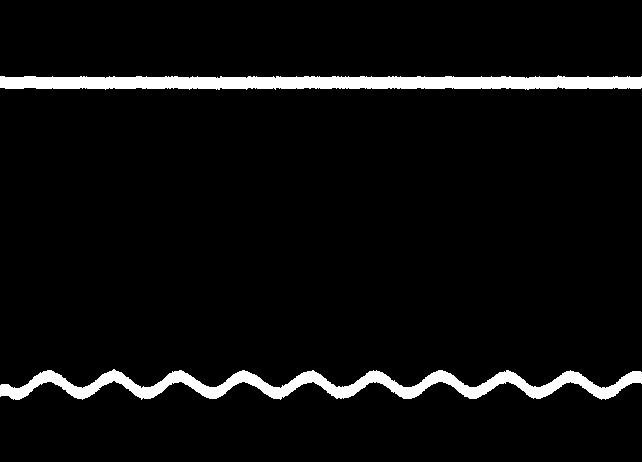
\includegraphics[width=\linewidth,angle=0]{imagenes/bandas22.10.21_A=3_L=21.png}
\caption[Bands example]{Image of the bands for the same mask shown in figure \ref{mask} c).}
\label{bands}
\end{wrapfigure}

\newpage

\subsection{Noise treatment}

As we said, the intensity values are given by $v_{ij}^t  = n_{ij}^t +  b_{ij}^t$. We are only interested in $b_{ij}^t$, and therefore, we want to minimize the effects of the noise. One important thing to consider is that the mean noise intensity is not the same for every pixel. In other words, the probability density function of noise intensities depends on space. There are two main reasons for this inhomogeneity. First, there are different noise levels at the PDMS and the MMA because out of focus bacteria contribute to the noise, and we can see in figure \ref{noise_img} a) and b) that the noise is higher on the liquid. Second, the illumination is inhomogeneous because we close the diaphragm to decrease noise intensity, only allowing light in the ROI to enter the camera, but the effect is more intense on the edges of the image. This effect is often less important than the first.

To deal with the dependence on space of $n_{ij}^t$, we exploit many properties of the data. We first approximate the noise distribution by just calculating the mean intensity of  $\bar{v} = \langle v_{ij}^t \rangle_{ijt}$ where the average is over space and time, as the lower indices indicate. Since for most pixels, the bacteria intensity $b_{ij}^t=0$ as bacteria occupy a small fraction of the ROI, $\bar{v}$ is slightly greater than the mean of $n_{ij}^t$ for different pixels. Now, we assume that every pixel satisfying $v_{ij}^t  < \bar{v} + 3 \sigma$ where $\sigma$ is the standard deviation of $v_{ij}^t$ do not include bacteria fluorescence, i.e. $b_{ij}^t =0$. The $v_{ij}^t$ values that satisfy the previous inequality are renamed as $N_{ij}^t$ because they represent an approximation of the noise. The histogram of $N_{ij}^t$ is shown in figure \ref{noise_img} c). Then, we are only interested in the region with MMA and bacteria, so we estimate the mean of the noise in that region:

\begin{equation} \label{eq:noise_aproximation}
	n_{est} \equiv {\rm mean_{ROI}}(N_{ij}^t).
\end{equation}

\afterpage{%
\begin{figure}[H]
	\centering
	\includesvg[scale=1]{imagenes/noise_example}
	\caption[Mean noise example]{ a) Mean noise image obtained averaging over time $V_{ij}^t$. The experiment displayed is one where the noise inhomogenities are clearly seen. b) Histogram of $V_{ij}^t$ over two $20 \times 500$ \SI{}{\square\pixels} windows, one in PDMS and the other on MMA. The noise distribution on MMA is shifted to the right compared with the one on PDMS. Also, the difference is greater toward higher values, probably due to the influence of bacteria out of the focal plane. c) Histogram of $V_{ij}^t$ only for pixels in the ROI. The ${\rm mean_{ROI}}$ function calculates the mean over this distribution. d) Histogram of $B_{ij}^t$, the video that is used for future measurements. The dashed black line is on $B=0$.  }
	\label{noise_img}
\end{figure}
}

Here the ${\rm mean_{ROI}}$ function represents the mean of the values of $N_{ij}^t$ for pixels in any frame but inside the ROI defined by the mask. The resulting $n_{est}$ is then substracted to the video so now the intensities on the video are given by $B_{ij}^t  = b_{ij}^t + \tilde{n}_{ij}^t$, where $\tilde{n}_{ij}^t  = n_{ij}^t - {\rm mean_{ROI}}(n_{ij}^t)$. The matrix $\tilde{n}_{ij}^t$ averages 0 in the ROI, therefore averages of $B_{ij}^t$ in time and space will only consider bacteria intensity.


\subsection{Intensity analysis}

The properties of the $B_{ij}^t$ matrix give the possibility to measure mean bacteria intensity over time and space identically as measured with $ b_{ij}^t$. We are interested in how bacteria behave in the bands of each wall and how both walls compare. To do so, we consider $M_{ij} = \langle B_{ij}^t \rangle_t $. The image $M_{ij}$ is called the mean image of the experiment and is an indicator of where bacteria swam through. An example of $M_{ij}$ is shown in figure \ref{mean_image_and_profile} a). Then we consider the intensity near a wall $i_i^y$ as:

\begin{equation}
	i_i^y = \sum_{j \in B_y} M_{ij},
\end{equation}

where $B_y$ is the band of a specific wall $y$. Then the definition of $i_i^y$ is the vertical sum of $M_{ij}$ over the band $B_y$. We normalize the intensity profiles by the mean of the flat wall intensity profile $\bar{i}^f = \langle  i_i^f\rangle_i $. 

\begin{equation}  
	\tilde{i}_i^y = \frac{i_i^y}{\bar{i}^f}.
\end{equation}

This normalization allows the comparison between different experiments respect to the standard of the flat wall. It also removes the problem of different bacteria intensities $b_{ij}^t$ due to fluorescence decay. 

The curved wall has a sinusoidal form, so it is reasonable to average $\tilde{i}_i^y$ over every period. If the experimental data has $N$ periods for the experiments whit amplitude $A$ and wavelength $\lambda$ then the intensity profile $I^y(x)$ of the wall $y$ with that shape is:

\begin{equation} \label{eq:Intensity profile}
	I^y(x) = \frac{1}{N} \sum_{n=1}^N \tilde{i}_{x+ n\lambda}^y.
\end{equation}

It is essential to clarify that the coordinate $x$ only takes values among one wavelength as the average is on every period and $x=0$ corresponds to the position of the valley. One set of profiles is displayed in figure \ref{mean_image_and_profile} b) as an example. The profile of the flat wall is obviously flat and equal to $1$ for all experiments, so it will never be plotted again. For simplicity, from now on we define $I(x)$ as the intensity profile of the curved wall, without the upper index $c$. Chapter 4 will profoundly discuss all the information and physics related to intensity profiles.


\begin{figure}
	\centering
	\includesvg[scale=1]{imagenes/mean_image_and_profile}
	\caption[Mean image and profile of an experiment]{a) Mean image $M_{ij}$ of a experiment. The accumulation on the walls can be seen. b) Normalized intensity $I(x)$ for both walls. The errorbars are the confidence interval of $95\%$ for the estimation of the mean $I(x)$ over the $N$ periods.}
	\label{mean_image_and_profile}
\end{figure}

\newpage

\subsection{Bacteria tracking}

\begin{wrapfigure}{r}{0.5\linewidth}
\centering
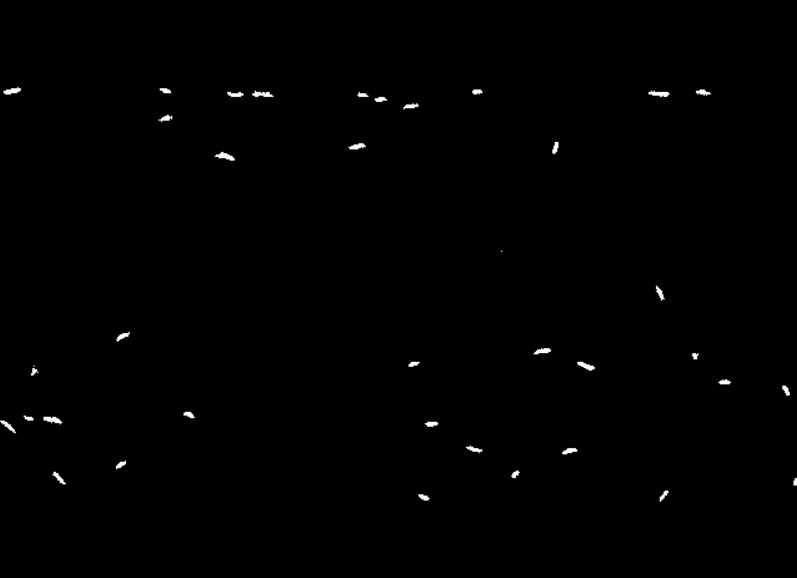
\includegraphics[width=\linewidth,angle=0]{imagenes/track_video_frame.PNG}
\caption[Tracking video frame]{Example of a typical frame for the binarized matrix $T_{ij}^t$.}
\label{tracking_video_frame}
\end{wrapfigure}


Tracking, in general, refers to determining the trajectories of objects in an image sequence. There are two main steps when doing the tracking: object detection and track creation. In the subsection, we will describe two different methods for doing detection and the tracking method based on linear assignment problems (LAP tracker). These methods are the ones that were the most succesful during this MSc thesis, but other options were studied as well. All of the methods that will be discussed are already implemented on Trackmate, an open-source plugin for Fiji \cite{Tinevez2017TrackMate:Tracking}. 


We start by describing object detection. The specific objective is to determine bacteria position via the intensity $B_{ij}^t$. Then, a detection algorithm should be able to measure intensity variations indicative of the presence of bacteria. One possibility is to use the Laplacian of Gaussian detector (LoG) \cite{Kong2013AApplications,Sage2005AutomaticDynamics}. This method is easier to understand if the matrix $B_{ij}^t$ is thought of as a scalar field $B(x,y,t)$. We only know the field values at a regular grid of point, but we can calculate integrals and derivatives using standard numerical methods. As the detector's name indicates, we first convolve with a Gaussian and then calculate the Laplacian of the result. The equations for the method are:  

\begin{align}
	G(x,y;\sigma) &= \frac{1}{\sqrt{2\pi \sigma^2}} \exp\left(  -\frac{x^2+y^2}{2\sigma^2} \right), \\
	B^{gb}(x,y,t;\sigma) &= B(x,y,t) * G(x,y;\sigma), \\
	R(x,y,t;\sigma)  &= \nabla^2 B^{gb}(x,y,t;\sigma). \label{LoG:result}
\end{align}

Here $G(x,y;\sigma)$ is a Gaussian kernel that, when convolved ($*$ operation) with the image, produces a polished version $B^{gb}(x,y,t;\sigma)$ where $gb$ stands for gaussian-blurred. The reason for this smoothing effect of this convolution is that it acts as a low-pass filter for the field \cite{WaltzaAnMachines}, removing highly space-dependent noise contributions. The value of $\sigma$ is $r/\sqrt{2}$ where $r$ is the estimated bacteria radius. More importantly, in equation \ref{LoG:result} the Laplacian operator $\nabla^2$ is applied to obtain $R(x,y,t;\sigma)$. The result is that bacteria with maximum intensity in the center will also have a minimum negative Laplacian there, so local minima in $R(x,y,t;\sigma)$ are bacteria centers. Locality, in this case, refers to a circle of the estimated radius $r$, so the method detects bacteria as blobs of that size. There are more generalized versions of LoG that allow the consideration of non-circular particles \cite{Kong2013AApplications}. This method is ideal for images with noise and particles with a maximum intensity at their center and decaying at a radius $r$, but it only detects circumferences, so it should not be used if it is necessary to know the exact shape of the particles.

Another possibility to consider is binarizing the videos. A binarized image will have sharp variations of intensity, and if done correctly, will not lose bacteria in the process. In our case, we again use Otsu's binarization method into the matrix $B_{ij}^t$. The result is then used for the tracking, so we call it $T_{ij}^t$. An example of a typical frame of this tracking video is shown in figure \ref{tracking_video_frame}. Bacteria detection in  $T_{ij}^t$ is straightforward because considering all connected regions as a particle is enough. This detection method is known as the thresholding detector. One possible issue is that there is only one detection when multiple cells collide. In figure \ref{detection_method_comparison} there is a comparison with results for the two methods. The LoG detector works well with noise, which does not mean that it will fail with a binarized image. Proper binarization often helps with any detection method. Conversely, the thresholding detector adapts to bacteria form and does not make fake detections. This last point convinced us to use a thresholding detector for these experiments.

\begin{figure}
	\centering
	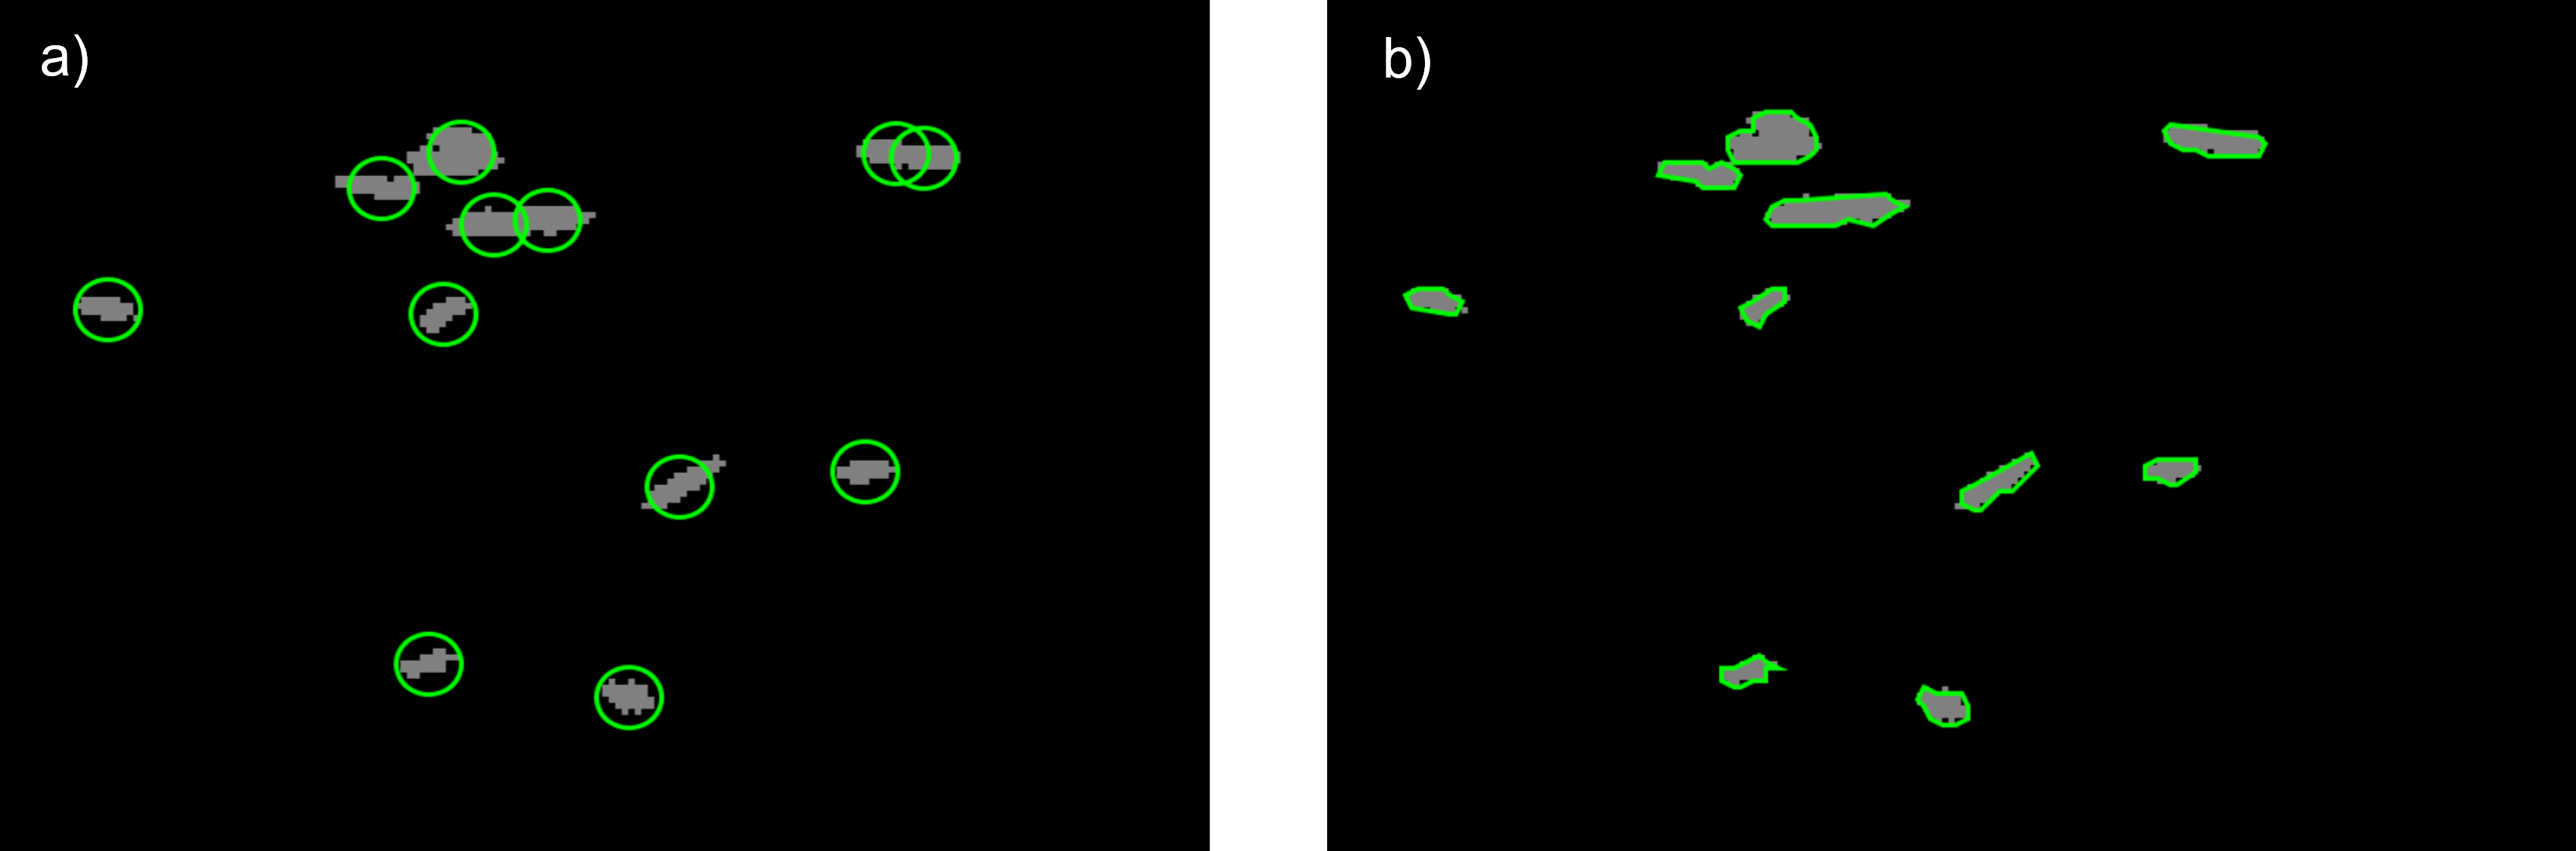
\includegraphics[width=\linewidth]{imagenes/detection_method_comparison.png}
	\caption[Detection method comparison]{ Zoom image of a video $T_{ij}^t$, and bacteria detection results displayed in green for a) LoG detector and b) Thresholding detector. LoG detector adds virtual detections in large bacteria, but the thresholding method will account for multiple bacteria collisions as only one particle. Methods give comparable results, but the best choice will depend on experimental properties, such as bacteria shape and frequency of collisions. In our case, Otsu's binarization method has the conditions to perform the algorithm successfully, so the overall thresholding detector has better results than the LoG detector. }
	\label{detection_method_comparison}
\end{figure}

Now we deepen into the automatic tracking method described in Trackmate's user manual. There are many options for automatic tracking that use simple criteria such as the nearest neighbor assignment or overlapping criteria. It is not meriting to explain these methods as they only work under restricted conditions. Instead, the idea behind LAP trackers gives a general tool for tracking without overcomplications \cite{Jaqaman2008RobustSequences}. A linear assignment problem refers to determining the assignment matrix A that satisfies:

\begin{equation}
  A = {\rm argmin} \left(  \sum_{k,l} A_{kl}C_{kl} \right),
\end{equation}

where $C_{kl}$ is a cost matrix and $A_{kl}$ is a boolean matrix of 1 (link) and 0 (no-link) with the restriction that there is only one link for each row or column. To understand how this problem is used for tracking we need to inspect the cost matrix $C$. The simpler form of $C$ is to consider connections between detections of two frames $t$ and $t+1$. These frames will have $n$ and $m$ detections, respectively. Then $C$ is an $(n+m) \times (n+m)$ with four quadrants. 

\begin{itemize}
	\item The top left quadrant of size $n \times m$ has the cost of linking a detection on frame $t$ to one in $t+1$. The cost is $C_{kl} = (D_{kl}P_{kl})^2$ where $D_{kl}$ is the distance between the detections and $P_{kl} = 1 + \sum_f p_{kl}^f$ where $p_{kl}^f$ is a penalization for differences on the particle feature $f$ given by $p_{kl}^f = W_f \frac{|f_k - f_l|}{f_k + f_l}$, where $f_k$ is the value of the feature $f$ for particle $k$. Features that are useful with the thresholding detector are bacteria perimeter and area. The usage of penalization by features requires these characteristics to be held constant for there to be a connection. The magnitude of the feature penalization $W_f$ regulates the importance of this conservation. If $D_{kl}$ exceeds the double of the mean distance traveled in each frame, $C_{kl}$ is set to infinity
	\item Top right and bottom left quadrants are cost for not linking particles for frame $t$ and $t+1$ respectively. The cost values are set to $c = 1.05 \times {\rm max}(C_{kl})$ where the maximum is only taken on the top left quadrant and does not consider the infinite values.
	\item The bottom right quadrant is an auxiliary matrix in the Munkres and Khum algorithm used to solve the LAP problem \cite{Munkres1957AlgorithmsProblems}.
\end{itemize}

Considering the form of the cost matrix $C_{kl}$, depending on the quadrant of the connections, the assignment matrix $A_{kl}$ will connect detections from one frame to another or start/end tracks. Applying this to all frames will create the trajectories of the particles. A similar LAP can be considered for all the resulting tracks. In this case, the goal is to merge tracks, so the cost matrix includes distances between ends and starts of tracks. The cost is infinite if the end occurs at a time $T$ before the start. This process is called gap closing, as it allows to solve gaps in the tracks caused primarily due to detection failures involved in collisions. If particles separate from each other soon after the collision, this process will fix the errors. If they do not, the involved particles could be interchanged, causing wrong links, so the time $T$ should be kept as low as possible.  The LAP tracker as both frame-to-frame linking and gap closing works for general-purpose tracking, but Brownian motion is the best performing case for this method.

Nevertheless, we used a more specific version of the LAP tracker that considers the trajectories' properties in our experiments. The modification is simple but has profound effects. Based on particle trajectory, a prediction of where spots will be in the next frame is made. Instead of linking detections to each other, detections are linked with predictions based on the previous frame. The Kalman filter, also known as the linear quadratic estimation algorithm, is used to make predictions. Kalman filtering is a world in itself and has applications in robotics, navigation of vehicles,  geophysics, among others \cite{Auger2013IndustrialReview,Aanonsen2009TheReview}. Here we need to know that the Kalman filter considers bacteria's previous velocities to predict the future positions. Predictions allow gap closing differently. If two particles collide, there will only be one detection for two tracks. Then, one prediction will not have a link, but another prediction can be made for the next frame based on the previous. Predictions can fail to link up to $N_f=4$ times before the track is ended. If a track successfully encounters a detection before the $N_f$ failed attempts, the gap is closed. However, the predictions are not registered as intermediate positions, only truly measured detections. This method has two more parameters: the initial search radius $r_i=\SI{15}{\pixels}=\SI{4.8}{\micro\meter}$ and the search radius $r_s=\SI{10}{\pixels}=\SI{3.2}{\micro\meter}$. Both are the maximum allowed distances for frame-to-frame linking, with the difference that $r_i$ is only for new track initiation while $r_s$ is for linking considering predictions. The algorithm is briefly summarized as:

\begin{itemize}
	\item In the first frame, particles are linked to the second frame using standard particle to particle connections. The result is many starting tracks whose initial velocity can be measured, so predictions via Kalman filtering are now possible.
	\item For subsequent frames, the LAP is changed to prediction to particle linking, but the cost matrix structure does not change. New velocity measures will be considered in the Kalman filtering predictions.
	\item If a track fails to connect its prediction to a detection, new predictions will be made for future frames based on the current prediction. If this fails up to $N_f$ times, the track is terminated.
	\item Also, new particles could appear, so if a detection fails to find a track, the next frame, that detection will be considered in a separate LAP for tracking initiation. This LAP will be solved only with particles not in a track and after solving the LAP with predictions. This assigning order means that a track creation can not cause other tracks to end.
\end{itemize}

The algorithm is successful in gap closing and frame to frame linking, bypassing problems caused by collisions. This affirmation only applies if particles have a roughly constant velocity and the search radius $r_s$ is more than the displacement between successive frames. The second point is important because when bacteria collide with a wall, they may completely stop, so a short $r_s$ may exclude these cases ending the track. All the results of tracking are left for Chapter 4; meanwhile, figure \ref{tracking_examples} shows some trajectory examples. In table \ref{table:image analysis parameters} all the relevant quantities for the methods described in this chapter are summarized.

\begin{figure}
	\centering
	\includesvg[scale=1]{imagenes/tracking_trajectories}
	\caption[Example of trajectories]{Example of trajectories obtained with the tracking method. The star represents the start of each track and the triangles the end of them. The mask is used as background to show the walls. Dimensions of the curved wall are shown at the bottom.}
	\label{tracking_examples}
\end{figure}


\begin{table}[!h]
   \centering
    \small
    \caption[Summary of all quantities used in the image analysis]{All the quantities used for the image analysis, with their description and values. Parameters that are discussed but not include in the methods are not included in thise table. }
    \begin{tabularx}{\textwidth}{lXl}
    \hline\noalign{\smallskip}
         Quantity  & Description & Values   \\
    \noalign{\smallskip}\hline\noalign{\smallskip}
         $A$ & Amplitude of the sinusoidal curved wall. & \sim \SIlist[list-units=single, list-final-separator = {, }]{3;6;9;12}{\micro\meter} \\ 
         $\lambda$ & Wavelength of the sinusoidal curved wall & \sim \SIlist[list-units=single, list-final-separator = {, }]{21;24;27;30}{\micro\meter} \\
         $v_{ij}^t$ & Intensity of the raw data in the video. & \quad \\
         $\bar{v}$ & Mean of the matrix $v_{ij}^t$. & \quad \\
         $\sigma$ & Standard deviation of the matrix $v_{ij}^t$. & \quad \\
         $b_{ij}^t$ & Part of the signal $v_{ij}^t$ associated to bacteria fluorescence. & \quad \\
         $n_{ij}^t$ & Part of the signal $v_{ij}^t$ associated to the background noise. & \quad \\
         $W_{ij}$ & Image with the max value of $v_{ij}^t$ for all frames. After binarization is the mask that defines the ROI of the experiment. & \quad \\
         $B_c$ & Band of the curved wall. Is the surface \SI{4}{\micro\meter} thick starting from the wall boundary into the ROI.  & \quad \\
         $B_f$ & Band of the flat wall. Is the surface \SI{4}{\micro\meter} thick starting from the wall boundary into the ROI.  & \quad \\
         $V_{ij}^t$ & Video data considering only values that satisfy $v_{ij}^t  < \bar{v} + 3 \sigma$. The mean of this matrix over the ROI is used to eliminate noise contributions.  & \quad \\
         $B_{ij}^t$ & The raw data $v_{ij}^t$ minus ${\rm mean_{ROI}}(V_{ij}^t)$. Averages of $B_{ij}^t$ are equal to one done exclusively with $b_{ij}^t$.  & \quad \\
         $M_{ij}$ & Mean image obtained as $\langle B_{ij}^t \rangle_t$  & \quad \\
         $i_{i}$ & Intensity near a specific wall, averaged over the vertical direction in the respective wall.  & \quad \\
         $I_{i}$ & Characteristic intensity profile in one period corresponding to the periodical average of $i_i$ (see equation \ref{eq:Intensity profile}).   & \quad \\
         $r_i$ & Initial search radius for the LAP tracker. Radius $r_i$ is used for particle-particle linking at the beggining of a track.   & \SI{4.8}{\micro \meter} \\
         $r_s$ & Search radius for a current tracking the LAP tracker. Radius $r_s$ is used for particle-prediction linking.    & \SI{3.2}{\micro \meter} \\
         $N_f$ & Number of allowed failures for particle-prediction linking before the track is ended. & 4 \\
    \hline\noalign{\smallskip}
    \end{tabularx}
    \label{table:image analysis parameters}
\end{table}

\chapter{Numerical models and simulations}

\section{Theoretical framework}

This section explains details of the numerical model considered and the criteria used for its election. We consider an agent-based model of spherical active particles with overdamped dynamics in a 2-dimensional representation. 

\subsection{Agent-based models} 

In biophysics, models can be sorted into two classes, agent-based, and continuum models. Agent-based models simulate the dynamics of cells individually, offering accurate system descriptions. Depending on the complexity of the model, they can be costly in a computational sense. On the other hand, continuum models consider a coarse-grained description with density and velocity fields. We work in a low-density regime, so a continuum description is meaningless. Therefore, we will use agent-based models. For simplicity, we consider cells with spherical shapes. In reality, the cell shape depends on the growth phase of the bacteria culture, but \textit{E.coli}'s body is a spherocylinder with typical dimensions of \SI{0.5}{\micro\meter} in radius and \SI{2}{\micro\meter} in length.

\subsection{Overdamped dynamics}

To describe the dynamics of single cells, we invoke Newton's second law: 

\begin{equation}
	m\ddot{\textbf{r}} = \sum \textbf{F} = \textbf{F}_{\text{hydro}} + \textbf{F}_{\text{flag}} + \textbf{F}_{\text{brown}} + \textbf{F}_{\text{coll}} ,
\end{equation}

where we define four different force sources, $\textbf{F}_{\text{hydro}}$ the hydrodynamic friction produced by the fluid, $\textbf{F}_{\text{flag}}$ the force produced by the flagella, $\textbf{F}_{\text{brown}}$ the Brownian force due to collisions with the liquid molecules, and $\textbf{F}_{\text{coll}}$ produced due to cell-cell and cell-surface collisions. We can deduce an important fact widely accepted in microscopic systems with the following analysis. To analyze the role of inertia, let's imagine we have isolated \textit{E.coli} bacterium that suddenly stops swimming, so $\textbf{F}_{\text{flag}} = \textbf{F}_{\text{coll}} =0$. Although the influence of $\textbf{F}_{\text{brown}}$ is essential, its effect is stochastic with zero mean. If we repeat the situation many times and average the ensemble, its contribution is expected to be zero. Therefore, for the moment, we will neglect it. Then we are left with the equation:

\begin{equation}
	m\ddot{\textbf{r}} = \textbf{F}_{\text{hydro}} = -\gamma \dot{\textbf{r}} = - 6 \pi R \eta \dot{\textbf{r}},
\end{equation}

where we used Stokes' law to calculate the drag force coefficient $\gamma$ with $R=$ \SI{0.5}{\micro\meter} being the particle radius and $\eta=$ \SI{d-3}{\pascal\cdot\second} the viscosity. Since the mass of an \textit{E.coli} is $m=$ \SI{d-12}{\gram}, the characteristic time of slowing down is given by $ m/(6 \pi R \eta) \approx $ \SI{d-7}{\second}. This means that in the timescale of \SI{1}{\micro\second} the bacteria should have stopped. We record at 10 fps in our experiments, so the detention is immediate for our time resolution. This means that we are working in the overdamped limit, where inertia is negligible, and so it is correct to simplify the dynamics as:

\begin{equation} \label{eq:overdamped_model}
	\gamma \dot{\textbf{r}} = \textbf{F}_{\text{flag}} + \textbf{F}_{\text{brown}} + \textbf{F}_{\text{coll}}.
\end{equation}

\subsection{Rotational diffusion}

We considered two different effects of the fluid in the bacterial dynamics. First, $\textbf{F}_{\text{hydro}}$ is a phenomenological dynamical drag force that represents the average effect of the liquid on an object moving through the fluid, and second, $\textbf{F}_{\text{brown}}$ of stochastic kind accounting for the thermal fluctuations. The latter produces a mean square displacement of $\langle r^2 \rangle (t) = 4 D t $ where $D$ is the diffusion constant given by the fluctuation-dissipation theorem \cite{Soto2016KineticPhenomena}:

\begin{equation}
	D = \frac{k_bT}{\gamma} \approx \SI[per-mode = symbol]{1.5d-1}{\square\micro\meter \per \second},
\end{equation}
 
where $k_b$ is the Boltzmann constant, $T$ the temperature of the fluid. The same value for $\gamma$ was used. This diffusion constant is purely translational. Nevertheless, the collisions between cells and water molecules also exert torques on the bacteria, meaning that the orientation of swimming is subject to an equivalent stochastic process. This process has a rotational diffusion constant $D_r$ independent of $D$. For smooth-swimming \textit{E.coli} it has been measured at $D_r=$ \SI[per-mode = symbol]{0.057}{\square\radian \per \second} \cite{Drescher2011FluidScattering}. We can perceive the importance of rotational diffusion by neglecting collisions in equation \eqref{eq:overdamped_model} and calculating the mean square displacement as described in \cite{Lauga2020TheMotility}.

\begin{equation} \label{eq:flagellar force}
	 \dot{\textbf{r}} =\frac{\textbf{F}_{\text{flag}} + \textbf{F}_{\text{brown}} }{\gamma} = u \textbf{p} + \textbf{F}^*_{\text{brown}},
\end{equation}

where $u=$ \SI[per-mode = symbol]{20}{\micro\meter \per \second} is the mean speed of bacteria, $\textbf{p}$ the vector of orientation, and $\textbf{F}^*_{\text{brown}}$ is just the force with the coefficient $\gamma$ absorbed. Integrating equation \eqref{eq:flagellar force} in time we obtain:

\begin{equation} \label{eq:positon}
	\textbf{r}(t) - \cancelto{0}{\textbf{r}(0)}  = \int_0^t [u \textbf{p}(t^\prime) +  \textbf{F}^*_{\text{brown}}(t^\prime)  ]dt^\prime ,
\end{equation}

Taking the dot product of \eqref{eq:flagellar force} and \eqref{eq:positon} we obtain an equation for the time derivative of the square displacement.

\begin{equation} \label{eq:derivative of msd}
	\dot{\textbf{r}} \cdot \textbf{r} = \frac{1}{2}\frac{d}{dt} (r^2) = \int_0^t  [u^2 \textbf{p}(t^\prime) \cdot \textbf{p}(t) + \textbf{F}^*_{\text{brown}}(t) \cdot \textbf{F}^*_{\text{brown}}(t^\prime)]dt^\prime + \text{irrelevant terms}.
\end{equation}


All the terms in the right side of equation \eqref{eq:derivative of msd} are stochastic and vary from cell to cell. Nevertheless, their average for all particles has properties that allow progress in the calculation. For example, the terms cataloged as irrelevant consider dot products of two quantities completely uncorrelated, the director vector $\textbf{p}$ and the force $\textbf{F}^*_{\text{brown}}$. Therefore after averaging on the ensemble of cells, the average dot product is zero, and we are left with: 

\begin{equation} 
	\frac{d}{dt} \langle r^2 \rangle &= 2 \int_0^t  \langle u^2 \textbf{p}(t^\prime) \cdot \textbf{p}(t) + \textbf{F}^*_{\text{brown}}(t) \cdot \textbf{F}^*_{\text{brown}}(t^\prime) \rangle dt^\prime.
\end{equation}


The quantity $\langle\textbf{p}(t^\prime) \cdot \textbf{p}(t)\rangle$ is the mean time correlation of the vector director \textbf{p} and depends on the rotational diffusion coefficient as $e^{-2D_r|t-t^\prime|}$ \cite{Lauga2020TheMotility}. On the other side $\textbf{F}^*_{\text{brown}}$ is assumed to be an uncorrelated noise, that satisfies $\langle \textbf{F}^*_{\text{brown}}(t) \cdot \textbf{F}^*_{\text{brown}}(t^\prime) \rangle = 2D\delta(t^\prime -t)$. Therefore, integrating over both $t$ and $t^\prime$ we obtain:


\begin{equation} 
    \langle r^2 \rangle (t) = \frac{u^2}{D_r}\left( t + \frac{e^{-2D_rt}}{2D_r} - \frac{1}{2D_r} \right) + 4Dt
\end{equation}

At short times,  $t \ll D_r^{-1} =$ \SI{18}{\second} the exponential can be expanded in a Taylor series $e^{-2D_rt}\approx 1 - 2D_rt + 2(D_r t^2) + \mathcal{O}(t^3)$ giving $\langle r^2 \rangle (t)  \approx (ut)^2$, which means that at short times particles swim is straight lines. Bacteria swimming is more important than diffusion even at our lowest time scale of $t=$ \SI{0.1}{\second}, as in that case $4Dt$ is two order of magnitude lower than $(ut)^2$. In the other case $t \gg D_r^{-1}$ the mean square displacement is $(u^2/D_r+4D)t$. Adding the translational diffusion discussed previously, we deduce an effective diffusion constant for long times $D_{\text{eff}}$ given by:

\begin{equation}
    D_{\text{eff}} = D + \frac{u^2}{4D_r}
\end{equation}

For the typical values mentioned, $D_{\text{eff}}\approx$ \SI[per-mode = symbol]{2d3}{\square\micro\meter \per \second} which is four orders of magnitude larger than $D$. This means that bacteria swimming makes translational Brownian motion irrelevant compared to the effects of rotational diffusion. We conclude that $\textbf{F}_{\text{brown}}$ can be set to zero for simplicity without losing relevant dynamics. We are left with the equation:

\begin{equation} \label{eq:final_model}
    \dot{\textbf{r}} = u\textbf{p} + \frac{1}{\gamma}\textbf{F}_{\text{coll}} = u\textbf{p} + \textbf{F}^*_{\text{coll}} ,
\end{equation}

where $\textbf{F}^*_{\text{coll}}$ absorbs the drag coefficient $\gamma$ and hence has units of speed.

\subsection{Alignment with the wall}
\label{section:steric alignment}

We observe that bacteria interacting with the curved and flat walls, suffer a torque that aligns them with the wall \cite{Bianchi2017HolographicBacteria}. This alignment has its origin on steric forces. If we consider equation \eqref{eq:final_model} and take the dot product with the vector perpendicular to the surface  $\hat{\textbf{n}}_w$ at the point of contact, we obtain:

\begin{equation} \label{eq:steric_force}
   \cancelto{0}{\dot{\textbf{r}} \cdot \hat{\textbf{n}}_w}  = u\textbf{p} \cdot \hat{\textbf{n}}_w + \textbf{F}^*_{\text{coll}} \cdot \hat{\textbf{n}}_w ,
\end{equation}

where $\dot{\textbf{r}} \cdot \hat{\textbf{n}}_w = 0$ is imposed as bacteria do not cross the surface. Since the collision force with the wall $\textbf{F}^*_{\text{coll}}$ is exclusively perpendicular to the wall, equation \eqref{eq:steric_force} gives the magnitude of the collision force as $\gamma u \textbf{p} \cdot \hat{\textbf{n}}_w$, where $\gamma$ reappeared because we are calculating the force. Then we can write the equation for the angle of swimming $\theta$ considering that the inertia of the cell is negligible and so that the sum of torques must be zero. Simplifying the system, we consider the torques respect to the center of mass as the rotational drag and the torque exerted by the wall. Other torques can be considered for more complete models to explain observations such as circular trajectories and longer residence times in the wall \cite{Lauga2006SwimmingBoundaries, Sipos2015HydrodynamicWalls}. For this thesis we decided to work with a simple model because these effects are not required to explain the abandonment of the curved wall by bacteria. Using equation \eqref{eq:steric_force}, 

\begin{equation} \label{eq:deduction_of_K}
    0 = - \gamma_r \dot{\theta} \hat{\textbf{z}} - u \gamma (\textbf{p} \cdot \hat{\textbf{n}}_w) (\textbf{r}_{cm} \times \hat{\textbf{n}}_w),
\end{equation}

where $\gamma_r$ is the rotational drag coefficient and $\textbf{r}_{cm}$ the vector from the center of mass to the point of contact, as we are calculating the torque with respect to the center of mass. Therefore, $\textbf{r}_{cm} \times \hat{\textbf{n}}_w = L_{cm} (\textbf{p} \cdot \hat{\textbf{t}}_w) \hat{\textbf{z}}$ where $\hat{\textbf{t}}_w$ is the tangential vector to the wall in the point of contact that satisfies $\hat{\textbf{z}} = \hat{\textbf{t}}_w \times \hat{\textbf{n}}_w$  and we used $\textbf{r}_{cm} = L_{cm} \textbf{p} $ with $L_{cm}$ is the distance between the center of mass and the point of contact taking into consideration the contribution of the flagella to the center of mass. The elements involve in these equations are shown in figure \ref{cp_wall_diagram}. We are left with the equations:

\begin{align}
    \textbf{p} &= \cos{\theta}\hat{\textbf{x}}+\sin{\theta}\hat{\textbf{y}}, \\
    \dot{\theta} &= -K (\textbf{p} \cdot \hat{\textbf{t}}_w)  (\textbf{p} \cdot \hat{\textbf{n}}_w) \Gamma(\textbf{r}, \textbf{p}),
    \label{eq:wall alignment}
\end{align}

where $K\equiv u L_{cm}\gamma / \gamma_r$. The scalar $K$ controls the intensity of the alignment and in ref. \cite{Bianchi20193DInterface} a fit of experimental data yields $K=$ \SI[per-mode = symbol]{4.9}{\radian \per \second}. In our study we consider $K$ as a free parameter with values between \SIlist[per-mode = symbol, list-units=single]{0;7}{\radian\per\second}. This is because we are considering the more complicated case of a curved wall. Also, $\Gamma(\textbf{r}, \textbf{p})$ is a step function that indicates if the bacteria is in contact with the wall or not. It is equal to $1$ when the distance from the center of the particle $\textbf{r}$ to the closest point of the wall is smaller than one radius, and its swimming direction points towards the wall i.e. $\textbf{p} \cdot \hat{\textbf{n}}_w < 0$ indicating the cell is going into the wall and not away from it. Otherwise $\Gamma$ equals zero.  Equation \eqref{eq:wall alignment} will align the vector $\textbf{p}$ with the $\pm\hat{\textbf{t}}_w$ depending on the sign of $\textbf{p} \cdot \hat{\textbf{t}}_w$. This effect is only considered for the flat and curved wall as the frontal wall is already taken into account because simulations are two-dimensional.

\begin{wrapfigure}{r}{0.5\linewidth}
\centering
\includesvg[width=\linewidth,height=4cm]{imagenes/cp_wall_diagram}
\caption[Diagram of the components involve in the wall allignment]{Diagram of the components involve in the wall alignment. $O$ represents the origin of coordinates.}
\label{cp_wall_diagram}
\end{wrapfigure}

We calculate the point of contact as the closest point in the walls to the cell by dividing the interval $[x-R, x+R]$ in 300 points where $x = \textbf{r} \cdot \hat{x}$. Then, we calculate the distance between the cell and the position obtained with the parametric definition of the wall for each point. The point $\textbf{r}_w$ with the lowest distance is the closest with a precision of \SI{3d-3}{\micro\meter}. This ``brute force" algorithm works because a point outside of the interval $[x-R, x+R]$ is not in contact with the cell, and it is convenient because the distance to the wall as a function of the $x$-axis has many local minima.

% \vspace{1cm}

\section{Simulations}

Equations \eqref{eq:final_model}--\eqref{eq:wall alignment} summarize the physics involved in the description of the system. We are only missing two aspects; rotational diffusion and the details of $\textbf{F}_{\text{coll}}^*$. This section first explains how we implement these phenomena, summarize the model, and finally explain how the simulations are performed.
 
\subsection{The collision force}

$\textbf{F}^*_{\text{coll}}$ is the force produced by the collision of cells with other cells or the wall, but divided by the drag coefficient $\gamma$. We considered it as an elastic force for both cell-cell and cell-wall collisions. We parameterize the force $\textbf{F}^{*,i}_{\text{coll}}$ that the $i$-th particle experiments through the following: 

\begin{equation}
   \textbf{F}^{*,i}_{\text{coll}} &= \sum_{w} k_{\text{wall}} (R-d_{iw}) \hat{\textbf{d}}_{iw}\Theta(R-d_{iw}) + \sum_{j \in \mathbb{NN}_i} k_{\text{cell}} (2R-d_{ij}) \hat{\textbf{d}}_{ij}\Theta(2R-d_{ij}),
\end{equation}
 
where $d_{iw}$, $\hat{\textbf{d}}_{iw}$ represent the distance and the unit vector between the particle $i$ and the closest point of the wall $w$, and $d_{ij}$, $\hat{\textbf{d}}_{ij}$ are the same but between the particles $i,j$ where $j$ is part of $\mathbb{NN}_i$ which is the set of nearest neighbors of the particle $i$. $\Theta$ is the usual Heaviside function. Finally the parameters $k_{\text{wall}}$, $k_{\text{cell}}$ are the intensities of these forces, and have units of \SI[]{}{\per\second}. We consider $k_{\text{wall}}=$ \SI[]{1d3}{\per\second}, which means that for $R-d_{iw}=$ \SI{2d-2}{\micro\meter} the magnitude of the interaction with the wall is equal to $u$, so it is impossible for bacteria to go through the surface. The parameter $k_{\text{wall}}$ is not related to $K$ it only defines the distance at which the elastic force is enough to repel bacteria. Meanwhile $k_{\text{cell}}$ will be considered as zero, meaning there are no cell-cell interactions. The explanation for such consideration is on section \ref{section: clustering}.

\subsection{Rotational diffusion}

 Rotational diffusion is naturally added to \eqref{eq:wall alignment} as a Gaussian white noise $\eta_i(t)$ \cite{Digregorio2018FullSeparation,Caporusso2020Motility-InducedSystem} meaning it has zero mean and its completly uncorrelated in time and between particles, $\langle \eta_i(t)\eta_j(t^\prime)  \rangle \propto \delta_{ij}\delta (t-t^\prime)$. This white noise will change randomly the direction of swimming $\textbf{p}$ of the cell. We will go into more detail in the following sections.
 
\subsection{Final model}

The final set of equations that are used in the model are:

\begin{align}
    \label{eq:dynamics of position}
    \dot{\textbf{r}}_i &= u\textbf{p}_i + \textbf{F}^{*,i}_{\text{coll}}, \\
    \textbf{p}_i &= \cos{\theta_i}\hat{\textbf{x}}+\sin{\theta_i}\hat{\textbf{y}}, \\
    \label{eq:dynamics of angle}
    \dot{\theta}_i &= -K (\textbf{p}_i \cdot \hat{\textbf{t}}_w)  (\textbf{p}_i \cdot \hat{\textbf{n}}_w) \Gamma(\textbf{r}_i, \textbf{p}_i) + \eta_i(t), \\
    \label{eq:elastic force}
    \textbf{F}^*_{\text{coll}} &=   k_{\text{wall}} (R-d_{iw}) \hat{\textbf{d}}_{iw}\Theta(R-d_{iw}) + \sum_{j \in \mathbb{NN}} k_{\text{cell}} (2R-d_{ij}) \hat{\textbf{d}}_{ij}\Theta(2R-d_{ij}).
\end{align}

All of the quantities used in these equations and on the model are described in table \ref{table:model parameters}. These equations are written for the dynamics of a circular particle $i$, involving other entities such as the wall and the nearest neighbors. Equations \eqref{eq:dynamics of position}--\eqref{eq:elastic force} belong to the class of Langevin equations due to their stochastic nature.

% Tabla del modelo
\begin{table}[!h]
   \centering
    \small
    \caption[Summary of the quantities used in the simulations]{Quantities used for the model, with their description and values if adequate. For parameters whose value changes, that column will have a $-$ symbol and in chapter 4, results will have that value specified. }
    \begin{tabularx}{\textwidth}{lXl}
    \hline\noalign{\smallskip}
         Variable  & Description & \quad   \\
    \noalign{\smallskip}\hline\noalign{\smallskip}
         \textbf{r} & Position of the particle $i$. & \quad \\ 
         \textbf{p} & Direction of swimming of the particle $i$, defined by the angle $\theta_i$. & \quad \\
         $\eta$ & White noise associated with rotational diffusion. & \quad \\
         $\hat{\textbf{t}}_w$ & Unitary vector tangent to the wall in the closest point to the cell $i$. & \quad \\
         $\hat{\textbf{n}}_{w}$ & Unitary vector normal to the wall in the closest point to the cell $i$. The normal vectors points away from the wall. & \quad \\
         $\hat{\textbf{d}}_{iw}$ & Unitary vector pointing from the closest point in the wall to the cell $i$. & \quad \\
         $d_{iw}$ & Distance between the cell $i$ and the closest point of the wall. & \quad \\
         $\mathbb{NN}$ & Set of nearest-neighbors of the particle $i$. & \quad \\
         $\hat{\textbf{d}}_{ij}$ & Unitary vector pointing from the neighbor $j$ to the cell $i$. & \quad \\
         $d_{ij}$ & Distance between the cell $i$ and the neighbor $j$. & \quad \\
    \hline\noalign{\smallskip}
        Parameter  & Description & Value   \\
    \noalign{\smallskip}\hline\noalign{\smallskip}
        $\rho$ & Density of cells. This density relates to the number of particles seen in the focal plane. & \SI[per-mode = symbol]{3d-3}{\cells \per \square\micro\meter} \\
        $u$ & Swimming speed. & \SI[per-mode = symbol]{20}{\micro\meter\per\second} \\
        $R$ & Radius of the cells. & \SI{0.5}{\micro\meter} \\
         $K$ & Magnitude of the aligment with the wall. & - \\ 
         $D_r$ & Rotational diffusion coefficient. & - \\ 
         $k_{\text{wall}}$ & Elastic constant for cell-wall collisions. & \SI{1d3}{\per\second}\\ 
         $k_{\text{cell}}$ & Elastic constant for cell-cell collisions. & 0 \\
         $\Delta t$ & Time step for the integration of the equations. & \SI{d-3}{\second} \\
         $\Delta t_r$ & Time step for the recording of data. & \SI{d-1}{\second} \\
         $T$ & Time duration of the simulations. & \SI{1200}{\second} \\
    \hline\noalign{\smallskip}
    \end{tabularx}
    \label{table:model parameters}
\end{table}

Quantities with the lower index $w$ depend on the wall. Simulations have a flat and a curved wall with amplitude $A$ and wavelength $\lambda$. The parametric definition of the walls positions are $y=y_f$ for the flat and $y=y_c+A\sin{\frac{2\pi x}{\lambda}}$ for the curved wall. The values of $y_f, y_c$ are so that the mean distance between walls is \SI{100}{\micro\meter}. Also, periodic boundary conditions will be applied. To avoid problems with discontinuities in the wall, the length of the channel is adjusted to have an integer number of wavelengths and be greater than \SI{300}{\micro\meter}. The total particle number is adjusted so that all simulations have the same particle density $\rho$. These values are similar to the experiments.

\newpage

\subsection{Numerical integration}

Typically, there are many options to solve a differential equation numerically. In this case, the equations are somewhat simple, so it is tempting to integrate \eqref{eq:dynamics of position} and \eqref{eq:dynamics of angle} with Euler's method. That integration method is a first-order method which means that during a step $\Delta t$ of integration, the integrands are taken as constants. Therefore we would obtain:

\begin{align}
    \textbf{r}_i(t+\Delta t) &=  \textbf{r}_i(t) + \Delta t[u \textbf{p}_i(t) + \textbf{F}^*_{\text{coll}}(t)], \\
    \label{eq:wrong integration}
    \theta_i(t+\Delta t) &=  \theta_i(t) + \Delta t[- K (\textbf{p}_i(t) \cdot \hat{\textbf{t}}_w)  (\textbf{p}_i(t) \cdot \hat{\textbf{n}}_w) \Gamma(\textbf{r}_i(t), \textbf{p}_i(t)) + \eta_i(t)].
\end{align}

However, there is a problem with the last term of equation \eqref{eq:wrong integration}, which relies on the timescale in which $\eta$ acts. Remember that $\eta$ represents the torque produced by collisions with the liquid molecules. These thermal fluctuations have a characteristic time between collisions of $\sim$\SI{1.9d-13}{\second} \cite{Soto2016KineticPhenomena}. That means we have two options, either we consider a minimal time step $\Delta t$ so the hypothesis that $\eta$ is constant in the interval is true, or we treat $\eta$ separately. The latter is the best option, as $\eta$'s timescale is much smaller than all the others present in the system. The correct equations are:

\begin{align}
    \textbf{r}_i(t+\Delta t) &=  \textbf{r}_i(t) + \Delta t[u \textbf{p}_i(t) + \textbf{F}^*_{\text{coll}}(t)], \\
    \theta_i(t+\Delta t) &=  \theta_i(t) - K \Delta t  (\textbf{p}_i(t) \cdot \hat{\textbf{t}}_w)  (\textbf{p}_i(t) \cdot \hat{\textbf{n}}_w) \Gamma(\textbf{r}_i(t), \textbf{p}_i(t)) \nonumber \\
     &\ \ \ + \int_t^{t+\Delta t}\eta_i(t^\prime)dt^\prime .
\end{align}


Then a new problem arises, how do we calculate the integral of $\eta$. We can find the answer on stochastic calculus, and here we describe one of the possible demonstrations. First, we treat $\eta$ as what it is, a discrete function representing all the collisions with liquid molecules.

\begin{equation}
    \int_t^{t+\Delta t}\eta(t^\prime)dt^\prime = \sum_{n=1}^N \phi\eta_n,
\end{equation}

where $\eta_n$ is proportional to the angle displacement produced in a certain collision $n$. The magnitude of these rotations is contained in $\phi$ so that we can treat them as standard normal Gaussians. As we stated, these collision displacements are also uncorrelated. Therefore, we can use that the distribution of the sum of two gaussian uncorrelated variables, $x\sim\mathcal{N}(\mu_x,\sigma_x^2)$ and $y\sim\mathcal{N}(\mu_y,\sigma_y^2)$, is given by $\mathcal{N}(\mu_x+\mu_y,\sigma_x^2+\sigma_y^2)$ and by induction obtain:

\begin{equation}
    \sum_{n=1}^N \eta_n \sim \mathcal{N}(0,N) = \sqrt{N}\mathcal{N}(0,1),
\end{equation}

were the last equality is in the sense of probability density distribution. Then, the total number of collisions $N$ is proportional to $\Delta t$, for instance $N=\alpha \Delta t$, where $\alpha$ is a rate of collisions. Then we can write:

\begin{align}
    \textbf{r}_i(t+\Delta t) &=  \textbf{r}_i(t) + \Delta t[u \textbf{p}_i(t) + \textbf{F}^*_{\text{coll}}(t)], \\
    \label{eq:correct integration}
    \theta_i(t+\Delta t) &=  \theta_i(t) - K\Delta t (\textbf{p}_i(t) \cdot \hat{\textbf{t}}_w)  (\textbf{p}_i(t) \cdot \hat{\textbf{n}}_w) \Gamma(\textbf{r}_i(t), \textbf{p}_i(t)) \nonumber \\
     &\ \ \ + \sqrt{\phi^2\alpha\Delta t} \eta(t).
\end{align}

Here $\phi$ is in \SI{}{\radian} and $\alpha$ in \SI{}{\per\second} so $\phi^2\alpha$ has units of \SI{}{\square\radian\per\second}, the same as the rotational diffusion coefficient. Therefore, we naturally obtained the diffusion coefficient, normally defined as $2D_r\equiv\phi^2 \alpha$. As already mentioned, for smooth swimmer \textit{E.coli} in liquids it has been measured that $D_r=$ \SI[per-mode = symbol]{0.057}{\square\radian \per \second}. Nevertheless we consider $D_r$ as a free parameter with values between $D_r=$ \SIrange[per-mode = symbol, range-units=single
]{0.001}{0.05}{\square\radian \per \second} as is expected to be lower in our case, due to the constraints of the walls. Therefore $K$ and $D_r$ are the free parameters of the model.

The result of equation \eqref{eq:correct integration} is really important for the consistency of the numerical integration, since the equation $\langle \eta(t)\eta(t^\prime)  \rangle &= \delta (t-t^\prime)$ implies that $\eta$ has units of \SI{}{\second^{-1/2}} so multiplying by $\Delta t$ instead of $\sqrt{\Delta t}$ is dimensionally wrong.


\subsection{Intensity profiles in simulations}


In experiments we construct intensity profiles using the intensity of bacteria fluorescence. In simulations there is no such thing, we can only measure bacteria positions $\textbf{r}_i$. Therefore, we have to measure the mean bacteria density. For each particle in the band of a wall $w$ we can assign a interval in the $x$-axis defined as $[x-\Delta x/2,x+\Delta x/2]$ where $x_i = \textbf{r}_i \cdot \hat{x} - x_{\text{valley}}$ is contained. Here $x_{\text{valley}}$ is the position of the nearest valley to the particle, meaning $x$ is on a interval of one wavelength $\lambda$ and $x=0$ is the position of the valley. This defines the mean bacteria density over a period $n^w(x)$ as the count of bacteria that were in contact with the wall $w$ in the interval defined by $x$. 

Obviously $n^w(x)$ is not the same as intensity profiles. To create a comparable quantity, we convolve $n^w(x)$ with a Gaussian function $G(x)=\exp(-x^2/(2R^2))$. We call the result the intensity near a wall $w$ for the simulation:

\begin{equation}
    i^w_{\text{sim}}(x) = n^w(x) * G(x).
\end{equation}

This treatment means we consider particles having a Gaussian intensity in space. This is not equal to the intensities measured in experiments because bactearia are not spherical. Nevertheless, treating intensity not spherically in simulations would lead to inconsistencies. The amplitude of the Gaussian does not matter as we will normalize by the mean accumulation in the flat wall. If the mean intensity on the flat surface is $\bar{i}^f_{\text{sim}} = \langle  i_{\text{sim}}^f(x)\rangle_x $. We define the normalized intensity profile in the curved wall as:

\begin{equation} \label{eq:Intensity profiles in simulations}
    I_{\text{sim}}(x) = \frac{i_{\text{sim}}^c(x) }{\bar{i}^f_{\text{sim}}}
\end{equation}

The normalized intensity profiles of simulations $I_{\text{sim}}(x) $ will be compared to the experimental result $I(x)$ in the chapter 4.

\newpage

\subsection{Algorithm}

The algorithm used in the simulations is described in the following steps.

\begin{itemize}
    \item[1.] Create a random initial condition for all the particles positions and swimming directions. If a particle is out of boundaries or in contact with a wall, its initial conditions are generated again. Then start iterating the time steps.
    \item[2.] Update the closest point of the wall for all particles close to the walls.
    \item[3.] Integrate the equation for $\theta_i$.
    \item[4.] Determine the $\mathbb{NN}$ set for all particles.
    \item[5.] Calculate the force $\textbf{F}^*_{\text{coll}}$.
    \item[6.] Integrate the equation for $\textbf{r}_i$.
    \item[7.] Every time interval $\Delta t_r$ record the relevant data. This avoids high time correlations between measurements.
    \item[8.] Stop when a time $T=$ \SI{1200}{\second} has passed.
\end{itemize}

The algorithm was implemented in a C++ program with object oriented programming. In figure \ref{sim trajectories} we display trajectories for the parameters $K=$ \SI[per-mode = symbol]{5}{\radian\per\second}, $D_r=$ \SI[per-mode = symbol]{0.05}{\radian\per\second} and $k_{\text{cell}}=0$.

\begin{figure}[H]
	\centering
	\includesvg[scale=1]{imagenes/sim_trajectories}
	\caption[Example of trajectories for the simulations]{Example of trajectories  obtained with the simulations for the parameters $K=$ \SI[per-mode = symbol]{5}{\radian\per\second}, $D_r=$ \SI[per-mode = symbol]{0.05}{\square\radian\per\second} and $k_{\text{cell}}=0$. The star represents the start of each track and the triangles the end of them. The values of $A$ and $\lambda$ are included on the top of the plot. Trajectories last for \SI{10}{\second}.}
	\label{sim trajectories}
\end{figure}

\chapter{Results}

This chapter is dedicated to the results obtained in experiments and the model. We start by describing the raw experimental results to get a big picture of the system. Afterward, we analyze intensity as an indirect measurement of the mean density accumulation, proving there is a transition in the accumulation near walls. Results of tracking explain further these observations.  

\section{Observations}
\label{section: observations}

In the introduction in Chapter 1, we discussed multiple effects of surfaces on bacteria. These effects appear depending on the swimming properties, body and flagella shape, and surface properties. In our experiments, we observe cell adhesion to the frontal wall when not using BSA, circular trajectories, non-zero contact angles with the flat walls causing trapping of bacteria in that wall, wall-cell alignment, and cell-cell interactions causing clustering.

\subsection{Cell adhesion}


We observe that cell adhesion to the frontal wall occurs when the surfaces are not coated with BSA. In figure \ref{adhesion} we show four frames of an experiment where BSA was not utilized. Four bacteria have adhered to the front wall. Adhesion gives rise to the biofilm formation that we want to avoid. In this case, the adhesion is of electrostatic origin and is therefore prevented by using BSA. It could be argued that using BSA affects the curved wall results in preventing adhesion and therefore should not be used. Nevertheless, we measure surface effects prior to adhesion to design a surface that allows bacteria to leave the wall. Once adhesion has occurred, bacteria will form biofilm independently of the shape of the surface. Therefore, this adhesion is not relevant to our measurements. In other terms, we are not studying cell adhesion mechanisms, so there are no reasons to measure this phenomenon. If we were measuring cell adhesion, to test our results, we should use wild-type strains where more adhesion mechanisms are present \cite{Costerton1987BacterialDisease.}. 

\begin{figure}
	\centering
	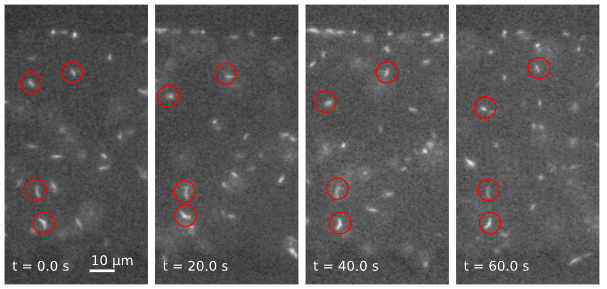
\includegraphics[width=\linewidth]{imagenes/adhesion.PNG}
	\caption[Frames of an experiment not used because the channel was not coated with BSA]{Four frames of an experiment where the channel was not coated with BSA. The four cells enclosed by red circles appear on all frames because they have adhered to the frontal surface. Adhered bacteria slightly move but never leave the focal plane. No measurements were made on these experiments. We only used them in this figure to show what happens when not using BSA. } 
	\label{adhesion}
\end{figure}


\subsection{Circular trajectories}

\begin{wrapfigure}{r}{0.5\linewidth}
\vspace{-50pt}
\centering
\includesvg[width=\linewidth]{imagenes/circular_trajectories}
\caption[Circular trajectories near walls]{Example of three circular trajectories observed in an experiment. The star indicates the beginning of a track while the triangle marks the end. The video used for this figure had 12 trajectories with circular sections of a total of 302, which correspond to $4\%$. The three shown trajectories are the longest ones.}
\vspace{-50pt}
\label{circular trajectories}
\end{wrapfigure}

We see circular swimming trajectories on the frontal surface, caused by hydrodynamic interactions between the cell and the boundary \cite{Lauga2006SwimmingBoundaries}. In figure \ref{circular trajectories} we display three example trajectories. The percentage of trajectories observed that display circular movement is $4\%$ for the experiment used for the figure. Thus, the phenomenon is marginal and, therefore, not implemented in the model. 

\label{section:cell trapping}
\subsection{Flat wall trapping}

Due to the hydrodynamic interactions when bacteria swim in contact with a flat wall, the angle of contact is not zero \cite{Sipos2015HydrodynamicWalls} as can be seen in figure \ref{trains}. This causes bacteria to swim along the surface in average for \SI{60}{\second} \cite{Drescher2011FluidScattering}. In our experiments, we observe this behavior in the two flat walls of the system, the upper and the frontal wall. Due to this effect, bacteria barely leave the focal plane, validating the two-dimensional aspect of the model. This effect has another interesting consequence. When swimming in contact with the wall, cells may encounter another cell swimming in the opposite direction, forming a pair of stagnant cells. Other cells that reach this pair will also become stagnant. After a time, typically in the order of 10 seconds, the cells manage to separate, and the bacteria that swim in the same direction leave together. This forms ``trains" of cells moving in the same direction as shown in the figure \ref{trains}. Usually, the observed trains have less than ten cells, and not all cells on the flat wall move in trains. 

 
\begin{wrapfigure}{r}{0.5\linewidth}
\centering
\includesvg[width=\linewidth]{imagenes/tren}
\caption[Observation of a train of bacteria swimming in the same direction]{Observation of a train of bacteria moving to the right in three different frames with their respective times $t$. We also see how the bacteria swim at a non-zero angle when in contact with the flat wall. The red line is the border of the ROI, representing the flat wall.}
\vspace{-50pt}
\label{trains}
\end{wrapfigure}

When a cell swimming in the opposite direction of a train collides with it, it moves into the focal plane or away from the upper wall. This occurs because the train has more mass and pushes harder than the individual bacterium displacing it. This effect causes bacteria to leave the flat wall. However, it is also possible that the bacteria do not interact with the train, as the system is three-dimensional.


\afterpage{
\begin{figure}[H]
	\centering
	\includesvg[width=\linewidth]{imagenes/trapping_merge}
	\caption[Trajectories of bacteria following the profile of the curved wall in experiments and simulation]{Four sequences of frames showing an individual bacteria going along the curve of a wall for $\lambda=$ \SI{30}{\micro\meter} and two different values of $A$, in experiments a,b) and simulations c,d). Each frame has the time $t$ on the bottom. The reference time $t=$ \SI{0}{\second} is exactly when the bacteria reach the wall. a) In this case, the amplitude is not too high, and therefore the bacterium can cross the valley in only \SI{1.5}{\second}. In the last frame, two bacteria appear, but it is clear which bacteria correspond to the previous frames if we consider the logical trajectory. b) For a higher amplitude, we observe that the bacterium stays in the same position for many seconds until it leaves. c, d) Results of simulations for  $K=$ \SI[per-mode = symbol]{3.0}{\radian \per \second}, $D_r= $ \SI[per-mode = symbol]{0.015}{\radian \per \square\second}. The arrow is the vector $\textbf{p}$. Trajectories and residence times in the simulations are similar to the experiments. The red line is the border of the ROI, representing the curved wall. }
	\label{esteric allignment}
\end{figure}
}

\subsection{Steric alignment with the wall}

When bacteria hit the wall, they experience a torque that aligns them with the wall, as described in section \ref{section:steric alignment}. For the flat wall, this effect means that after about 1 second, the bacteria are aligned with the wall. Aligned means that the bacterium swims with a stable non-zero angle, as mentioned in section \ref{section:cell trapping}. On the other hand, the effect is much more interesting for the curved wall and it depends on the values of the amplitude $A$ and the wavelength $\lambda$. We remember that $A$ and $\lambda$ have units of \SI{}{\micro\meter}. In figures the units will be omitted for simplicity. The torque allows the bacteria to follow the profile of the wall. Hydrodynamic interactions can cause bacteria to follow convex walls such as peaks \cite{Sipos2015HydrodynamicWalls}, but for the curvatures we are working with, this is rarely observed. Therefore, once they reach a peak, they stop feeling the steric torque and leave the wall. Only for $A=$ \SI{2.9}{\micro\meter} and $\lambda=$ \SI{30}{\micro\meter} some bacteria follow the sinusoidal shape of the wall. However, for high values of $A$ and low wavelength $\lambda$, bacteria could be trapped in the valley for a considerable time. This entrapment of cells in the curved wall can be due to a couple of reasons. In the case where there is only a single point of contact, we can understand this phenomenon by looking at the equation \eqref{eq:wall alignment}. For curved walls with high curvature, the vectors $\hat{\textbf{t}}_w$ and $\hat{\textbf{n}}_w$ vary significantly in space. This implies that as the bacteria swims parallel to the valley, the value of the dot product $\hat{\textbf{n}}_w \cdot \textbf{p}$ will stay close to zero even if the bacteria rotates. This causes the bacteria to rotate slowly and stay in the valley for longer times. Also, in the most extreme cases, corresponding to high $A$ and low $\lambda$, the bacteria may have several contact points with the wall, both with the body and the flagella, resulting in the bacteria being unable to rotate at all. 

In the figure \ref{esteric allignment} a, b) we show two individual cells whose trajectories illustrate the previously described phenomena. In sequence a) the amplitude is small enough for bacteria to move along the valley in \SI{1.5}{\second}. This is precisely what we are looking for. If bacteria can follow the wall curve and leave it in an interval of time lower than the characteristic adhesion time, we could reduce biofilm formation. In contrast, sequence b) shows how a bacterium spends too much time in the valley due to the reasons previously discussed. This will undoubtedly lead to adhesion in an in vivo environment. In the following sections \ref{section:intensity} and \ref{section: tracking} we will further investigate the behavior of bacteria on these surfaces by measuring the average density and speed when in contact with the wall. 

In simulations we observe a similar behavior. In figure \ref{esteric allignment} c, d) we show trajectories of particles with the parameters $K^*=$ \SI[per-mode = symbol]{3.0}{\radian \per \second} and $D_r^*= $ \SI[per-mode = symbol]{0.015}{\radian \per \square\second}. In section \ref{section:intensity} we will compare different values of $K$ and $D_r$ and it will be clear why these values were chosen for this figure. For now, we can observe that the model replicates the behavior in the valley, and also quantitatively the times are in the same order of magnitude. 


\label{section: clustering} 
\subsection{Clustering}

The phenomenon of bacteria trapping in the curved wall observed in figure \ref{esteric allignment} b) can be significantly increased when bacteria collide in the valley. For multiple bacteria colliding in one valley it is impossible for them to reorient and leave the wall. This will increase adhesion and the formation of biofilm. In figure \ref{clustering} we show two clusters of bacteria in a valley that were formed in the most extreme cases of amplitudes. The valley is very narrow, so bacteria stay in it for around \SI{10}{\second} even if alone. When other bacteria reach the valley, their movement is further restricted, and they cannot leave the wall. These clusters will last for several seconds, in some cases even for the entire video duration. We show representative examples where the clusters grow but also, sometimes, the cluster lose bacteria and even dissolve. Nevertheless, in a more natural environment, bacteria will adhere and then divide, and therefore biofilm will form. 

It is important to mention that this situation also occurs in walls with smaller amplitude, only less frequently. In figure \ref{cluster with low amplitude}, we show a case where this occurred for $A=$ \SI{2.9}{\micro\meter} and $\lambda=$ \SI{27}{\micro\meter}. Two bacteria collide and start a cluster, but shortly after, the cluster is dissolved when at time $t= $ \SI{13}{\second} two cells approach the cluster. These cells push the cluster causing all bacteria to align and leave the surface, as seen in  $t= $ \SI{14}{\second}. Cell-cell interactions play an important role in the dynamics of the system. We observe that cell-cell alignments can cause bacteria to leave or become trapped on the surface. The main difference between the cases of figures \ref{clustering} and \ref{cluster with low amplitude} is the effect that the cell-wall interaction produces. Cell-wall interactions could trap bacteria for several seconds if the valley is too narrow. Other bacteria will reach the valley, and a cluster will form, leading to residence times around \SI{100}{\second}. On the contrary, if cell-wall alignment contributes to bacteria leaving the wall quickly, cell-cell interactions are more infrequent and interrupt bacteria for less time, and therefore the accumulation in the surface will be reduced. The contribution of the steric alignment with the wall is the key to controlling accumulation on the surface.

\begin{figure}[H]
	\centering
	\includesvg[width=\linewidth]{imagenes/clustering}
	\caption[Clusters formed in valleys of the most ]{Clusters of bacteria formed in narrow valleys. Multiple bacteria collide and interrupt their movement, causing extremely long residence times. In both cases, $t=0$ corresponds to when the cluster was formed. a) The cluster was formed when two bacteria arrived almost simultaneously at a valley already occupied by a trapped cell. The cluster does not dissolve as the video ends in $t\sim$ \SI{130}{\second} and two bacteria remain in the valley. b) Another example where the cluster lasted for more than \SI{100}{\second} until it dissolved. The red line is the border of the ROI, representing the curved wall.}
	\label{clustering}
\end{figure}

\begin{figure}[H]
	\centering
	\includesvg[width=\linewidth]{imagenes/collison_low_A}
	\caption[Collision in a curved wall with low amplitude]{Example of a collision in a curved wall with a low amplitude. The residence time of bacteria involved in the collision is about \SI{10}{\second} while in figure \ref{esteric allignment} a) we observe a residence time of \SI{1.5}{\second} for a even more curved wall. The red line is the border of the ROI, representing the curved wall. }
	\label{cluster with low amplitude}
\end{figure}

\afterpage{
\begin{figure}[H]
	\centering
	\includesvg[width=\linewidth]{imagenes/clustering_simulation}
	\caption[Comparison in simulations between values of $k_{\text{cell}}$ in the high curvature case]{Comparison in simulations between values of $k_{\text{cell}}$ in the high curvature case. a) case with $k_{\text{cell}}=0$. In $t=$ \SI{0}{\second} three particles reach the valley, at $t=$ \SI{46}{\second}, more particles arrived on earlier frames but also particles start leaving the valley, independently of each other. The valley is empty at $t=$ \SI{65}{\second}. b) case with elastic interactions $k_{\text{cell}}=$ \SI{500}{\per\second}. In  $t=$ \SI{0}{\second} an initial bacterium occupies a valley and at $t=$ \SI{16.5}{\second} a second bacterium arrives. The collision between these two cells fixes the value of the the vector $\hat{\textbf{t}}_w$ to which bacteria align, allowing bacteria to leave only \SI{4}{\second} after the collision. }
	\label{clustering simulation}
\end{figure}}

\newpage

On the other hand, we consider an elastic interaction between the cells in the simulations. This interaction makes sense for spherical particles; however, it is not enough to capture what happens when clusters form in the valleys of the curved wall. The alignment between cells is relevant to describe cluster formation. When several bacteria collide in a valley, they disrupt each other and cannot follow the curve of the wall. In the figure \ref{clustering simulation} we show two simulation results for $A=$ \SI{10}{\micro\meter}, $\lambda=$ \SI{21}{\micro\meter} for two values of the elastic cell interaction $k_{\text{cell}}=$ \SIlist[list-units=single]{0;500}{\per\second}. In the case without interactions, bacteria reach the valley and share a similar position. The trapping time is large and around \SI{50}{\second}. The moment bacteria leave the cluster is completely independent of the other cells. Therefore, this is not a cluster of bacteria, but rather individual bacteria trapped for long times. The problem is that when we consider an interaction between cells, a meaningless dynamic appears. If two bacteria meet in the valley, the elastic force immobilizes both bacteria, which means that the vectors $\hat{\textbf{t}}_w$ and $\hat{\textbf{n}}_w$ remain constant for each bacterium. In a short time interval, both cells align with the vector $\hat{\textbf{t}}_w$ so they can leave the wall. The situation were $\textbf{p}\cdot\hat{\textbf{n}}_w \approx 0$ is broken by the collision of bacteria. 

We conclude that the model will underestimate the accumulation in the valley for cases with high curvature because it does not predict cluster formation. The best scenario for the model is to consider $k_{\text{cell}}=0$, so bacteria only accumulate due to the correctly modeled trapping in the valley. Since we are working on a low-density regime in experiments, we think that this simplification is plausible. This means that the optimal values of the model may not be applicable for high-density regimes where clustering forms more frequently. A more complicated model should consider cell-cell alignment to reproduce the clustering phenomena in the valley correctly. We will try to implement those interactions before publishing this work.
 
\label{section:intensity}
\section{Mean intensity}

The methodology described in section \ref{section: noise remove} allows us to consider the signal measured as coming solely from the fluorescence of the bacteria. Therefore the mean intensity registered in the experiments is an indirect measurement of bacteria density. We will measure mean intensity over a period. We begin by showing examples of the two-dimensional mean intensity and the effects of the previous observations in this quantity. Afterward, we describe intensity profiles $I(x)$ for the curved wall. These profiles exhibit a transition in their behavior that corresponds to what was observed in the section \ref{section: observations}. This will allow us to quantify the qualitative behavior exhibited by the system due to the alignment with the wall. 

\afterpage{
\begin{figure}[H]
	\centering
	\includesvg[width=\linewidth]{imagenes/2d_density}
	\caption[Mean intensity over a period for different values of $A$ and $\lambda$]{Mean intensity over a period $D_{xj}$ for different values of $A$ and $\lambda$. We choose the extreme values $\lambda =$ \SIlist[list-units=single]{21;30}{\micro\meter}. The brightness and contrast of the color scale was adjusted to improve the image display.  }
	\label{2d density}
\end{figure}
}

\subsection{Two-dimensional mean intensity}

We begin by showing results for $D_{xj}$ as defined in equation \eqref{eq:2d density}. $D_{xj}$ is the mean intensity over a period. In figure \ref{2d density} we show mean intensities over a period of the curved wall, for experiments with $\lambda =$ \SIlist[list-units=single]{21;30}{\micro\meter} and three different amplitudes. First, we note that intensities are not directly comparable between experiments, either because there is a different number of bacteria or because the bacteria fluoresce less intensely due to prolonged exposure. It is important to compare considering this aspect.

Nevertheless, it is clear that bacteria accumulate on the flat wall in all cases, but on the curved wall, the behavior depends on $A$ and $\lambda$. For low values of $A\approx$ \SI{3}{\micro\meter}, the curved surface presents fewer bacteria than the flat surface, as bacteria leave the wall when they reach a peak. As we increase the amplitude, we see how bacteria become trapped in the valley and eventually form clusters with high intensity. We call this transition the accumulation transition. The value of $A$ at which the bacteria become trapped depends on the wavelength $\lambda$ as can be seen when comparing experiments with similar amplitude \ref{2d density} b) and d). For all $\lambda$ we can observe the accumulation transition, meaning that at least there is an amplitude in which bacteria are trapped and another in which they are not.

These graphs also allow us to observe how the bacteria behave once they come out of the wall. In graphs b), e), and in particular f), it is possible to observe a darker zone near the valley. This is because once the bacteria leave the valley, they are unlikely to pass through this zone, as the angle at which they leave the wall is high. In the low amplitude case, a) and d), the amplitude is such that the bacteria stay close to the wall zone, and therefore this zone of depletion is not observed. Finally, in figure c) we observe that the curved wall only presents a high intensity on the valley. This means that clustering occurs, and so bacteria barely leave the valley, corresponding to the dynamics observed in \ref{section: clustering}. 

We observe that the average intensity captures various effects caused by the dynamics of the system. Accumulation on the flat wall, valley stagnation, and cluster formation. This reaffirms the usefulness of analyzing the average intensity to understand the system. The fact that the average intensity manages to capture the dynamics of the system should not be a surprise, as this is an indirect measure of bacteria density. 





\afterpage{%
\begin{figure}[H]
	\centering
	\includesvg[width=\linewidth]{imagenes/experimental_profiles}
	\caption[Experimental intensity profiles]{Experimental normalized intensity profiles $I(x)$ for a) $\lambda= $\SI{30}{\micro\meter} and b) $\lambda=$ \SI{24}{\micro\meter} with three different amplitudes. The colors were chosen so that curves associated with similar values of $A$ share color. The amplitudes that are shown allow to see the accumulation transition. Errorbars are the confidence interval of $95\%$ for the estimation of the mean $I(x)$. }
	\label{experimental profiles}
\end{figure}
}

\subsection{Intensity profiles}

The mean intensity matrix $D_{xj}$ has enough information to describe the system. Nevertheless, it also has two problems. It is not easy to compare due to differences in intensities between experiments, and it contains information of the bulk in the system that is not relevant for the measure of accumulation in the surface. Therefore, we consider the normalized mean intensity profiles $I(x)$ defined by equations \eqref{eq:Intensity profile} and \eqref{eq:Intensity profiles in simulations} for experiments and simulations respectively. These profiles are an average of the intensity in a zone \SI{4}{\micro\meter} normalized by the mean intensity in a \SI{4}{\micro\meter} thick zone from the flat wall. Thus, $I(x)$ indirectly measures the mean bacteria density in contact with the curved wall as compared to the flat wall. Experiments performed on different days do not show exactly the same profiles, as motility and density vary slightly, but thanks to this normalization, they are comparable. Therefore the average profile can be taken over all the experiments with the same curved wall parameters $A$, $\lambda$.   

In figure \ref{experimental profiles}, we show examples of experimental intensity profiles for $\lambda=$ \SI{30}{\micro\meter} and $\lambda= $ \SI{24}{\micro\meter} for three different amplitudes $A$. For low values $A$, the wall is slightly curved, and bacteria can move along it easily. The curvature makes bacteria leave the wall, therefore, the normalized intensity values are lower than 1. Also, there is a minimum at $x=0$ corresponding to the valley of the curved wall. This minimum is produced because not all cells touching the wall will go through the valley. If the contact starts near a peak, the cell will leave the wall without going through the whole period. Then, we have a critical amplitude, where $I(x)$ looks flat, which can be seen for $A=$ \SI{8.5}{\micro\meter} and $\lambda= $ \SI{30}{\micro\meter}. In this case, bacteria are still moving quickly around the wall, as the intensity is lower than the flat wall. Moreover, the intensity is lower than the previous case because bacteria leave the wall at a greater angle with respect to the wall axis. Finally, if the valley is too narrow, the intensity will greatly increase as bacteria get trapped. The more narrow the valley is, the higher the intensity peak as bacteria get trapped for longer times.

We can see how the profiles depend on both $A$ and $\lambda$ and conclude that $I(x)$ captures the accumulation transition successfully. This is relevant because we are considering less amount of data, but we are still representing the system correctly. We now present a quantitative description of the accumulation transition via the intensity profiles.

\subsection{The $c_1$ coefficient}

Qualitatively, the accumulation transition can be described as going from fewer bacteria in the valley of the wall to bacteria accumulating in there. This is represented by going from a minimum to a maximum at $x=0$. To quantify that aspect, we used the Fourier coefficient $c_1$ of the mean normalized intensity profile $I(x)$, calculated as:

\begin{equation}
    c_1 = \frac{2}{\lambda}\int_{-\lambda/2}^{\lambda/2} I(x)\cos\left(\frac{2\pi x}{\lambda} \right)dx = \frac{2}{\lambda} \sum_i I(x_i) \cos\left(\frac{2\pi x_i}{\lambda} \right)\Delta x,
\end{equation}

where $\Delta x=$ \SI{0.32}{\micro\meter} is the spatial resolution of the profiles and $x_i$ is the $i$-th position in the profile. Negative values of $c_1$ indicate a minimum on $x=0$ and positive $c_1$ the opposite.

\afterpage{%
\begin{figure}[H]
	\centering
	\includesvg[width=\linewidth]{imagenes/c1}
	\caption[Coefficient $c_1$ for experiments and simulations]{Color plots of the $c_1$ coefficient in the $A$, $\lambda$ parameter space. The colors are such that $c_1=0$ corresponds to the gray color and extreme negative and positive values are blue and red, respectively. a) Experimental results for $c_1$, where the number above each point represents the total number $N$ of periods considered in the average of equation \eqref{eq:Intensity profile}. b)--f) plots correspond to results from numerical simulations with their respective parameters indicated on the label. See text for more details. }
	\label{c1 coefficient}
\end{figure}
\newpage
}

Figure \ref{c1 coefficient} shows color plots of experiments and simulations for $c_1$ in the  ($\lambda$, $A$) parameter space, with red points representing an accumulation of bacteria in the valleys of the wall and blue points representing depletion of bacteria from the valleys. The transition from negative to positive values is seen in gray. The dashed line represents a two-dimensional interpolation of the curve where $c_1=0$, using an adapted version of the marching squares algorithm for irregular grids. We call the curve where $c_1=0$ the critical curve. In experiments, we can see how the accumulation transition occurs near $A= $ \SI{8.5}{\micro\meter}, $\lambda=$ \SI{30}{\micro\meter} and $A=$ \SI{5.6}{\micro\meter}, $\lambda= $ \SI{27}{\micro\meter}, but for the other wavelengths we lack the resolution in the amplitude to observe the critical amplitude $A$. We only know that it happens between $A=$ \SI{3}{\micro\meter} and \SI{5}{\micro\meter} as the dashed line indicates. 

In simulations, we show results for five different pairs of parameters $K$, $D_r$.  We remember that units of $D_r$ and $K$ are \SI[per-mode = symbol]{}{\square\radian\per\second} and \SI[per-mode = symbol]{}{\radian\per\second}, respectively. Units will not explicitly accompany values of the parameters for simplicity. In figure \ref{c1 coefficient} b) the pair of parameters $K^*=3.0$ and $D_r^*=0.015$ is the best fit for the values of $c_1$. We calculated the best fit as the set of parameters with the least square error compared to the experiments, without considering the experiments with $A\approx$ \SI{9}{\micro\meter}. We excluded those experiments because they have the least amount of realizations and show strange values of $c_1$ specially for $A= $ \SI{7.9}{\micro\meter}, $\lambda=$ \SI{21}{\micro\meter}. We only have experiments performed on a single day for those values of $A$. Unfortunately, our camera suffered a technical problem that produces condensation due to air infiltration into the sensor chamber. The camera is not available for new experiments in the mid-term. If these experiments are considered in the fit, the optimal pair only changes $D_r$ to $D_r^*=0.01$, but the fit is clearly worse.

Figures \ref{c1 coefficient} c) to f) demonstrate that not all pairs of parameters $K$, $D_r$ represent the accumulation transition trivially and also provide a notion of what results when varying the parameters. In c) and d) we use the same value of $D_r^* =0.015$ and change $K$. The case c) where $K=1.5$ predicts the critical curve for lower amplitudes than b), while d) the opposite. The interpretation is direct because $K$ controls the intensity of the alignment. Higher $K$ means bacteria move more easily along the valley and therefore are trapped less time, meaning the critical curve occurs at higher curvature. In contrast, figures e) and f) show what happens when $K^*=3.0$ is fixed and $D_r$ changes. When we increase the value of $D_r$ the transition occurs for lower amplitudes. This is because a higher thermal noise interrupts the alignment process. Nevertheless, when comparing the values of $c_1$ in $A= $ \SI{10}{\micro\meter}, $\lambda=$ \SI{21}{\micro\meter} we observe that increasing $D_r$ reduces that value. When cell trapping in the valley occurs, the steric torque is almost zero because bacteria are nearly perpendicular to the surface for a long time. Therefore, thermal noise can contribute to rotating bacteria more and reduce the residence time. Depending on the values of $A$ and $\lambda$, the coefficient $D_r$ may or may not contribute to the alignment to the wall.  



\begin{wrapfigure}{r}{0.5\linewidth}
% \vspace{-50pt}
\centering
\includesvg[width=\linewidth]{imagenes/c1_candidates}
\caption[Comparison of the accumulation transition curves for different values of $K$ and $D_r$]{Critical curves for different candidates compared to the experimental critical curve. The $c_1$ values correspond to the experimental values. We observe a parabolic shape for the critical curve. }
% \vspace{-50pt}
\label{c1_candidates}
\end{wrapfigure}


We conclude that $K$ and $D_r$ have opposite effects for the accumulation transition. Higher values of $K$ mean that bacteria align with the wall more quickly, but higher $D_r$ introduces more thermal noise that can make bacteria rotate bacteria against the wall alignment. Considering this opposite effect, many combinations of $K$ and $D_r$ can replicate the critical curve. We will call candidates, such pairs of $K$ and $D_r$ that replicate the critical curve similar to \ref{c1 coefficient} b). In figure \ref{c1_candidates} we show the critical curves for four candidates, compared to the experiment. None of the candidates exactly replicate the critical curve, specially due to the value $c_1=0.02$ for $A=$ \SI{8.5}{\micro\meter} and $\lambda= $ \SI{30}{\micro\meter} in experiments.

To understand this better, figure \ref{candidates intensity profiles} shows intensity profiles obtained in simulations of candidates, compared to the measured in experiments for values of $A$ and $\lambda$ that are of interest for the transition. The experiment's intensity profiles are subject to various effects that the simulations do not capture. For example, some experimental profiles are asymmetric due to inhomogeneities in density, causing more bacteria to come from one side, as observed in g), h), and i). However, this is not the only significant difference. In profiles d), e), and f), we see that the simulations do not predict a drop in the intensity values when the accumulation transition occurs; only the shape of the profile is adequately predicted, especially by the $K^*=3.5$, $D_r^*=0.015$ case. The experimental intensity profiles reach near-zero negative values for these cases, probably because we overestimated the mean noise for these cases. Also, in c), the experimental profile is flat, so $K=5.0$ is the closest curve, differing from the previous case.

\afterpage{
\begin{figure}[H]
	\centering
	\includesvg[width=\linewidth]{imagenes/candidate_profiles}
	\caption[Comparison of intensity profiles within experiments and four simulation candidates]{ Normalized intensity profiles for experiments and four simulation candidates. Rows have similar amplitude $A$, and columns have the same wavelength $\lambda$. The horizontal and vertical scales are adjusted depending on the amplitude and wavelength to pursue a clear display of the data. We only show representative candidates as many values represent the transition. Experimental error bars are the $95\%$ confidence interval for estimating the mean normalized intensity $I(x)$. The complete set of normalized intensity profiles is in appendix A. }
	\label{candidates intensity profiles}
\end{figure}
\newpage

\begin{figure}[H]
	\centering
	\includesvg[width=\linewidth]{imagenes/c1_curvature2}
	\caption[Coefficient $c_1$ as function of the curvature $\kappa$]{ Comparison between $c_1$ values for experiments and simulations with the best set of parameters. The dots enclosed by red circles correspond to $A\approx$ \SI{9}{\micro\meter} and were not considered for the fit. The inset is a close up to the low values of $\kappa$. The dashed line of the inset corresponds to $c_1=0$}
	\label{c1 curvature}
\end{figure}
}

We conclude that there is no perfect candidate to replicate the exact results of all experiments. A possible solution is to redefine the parameter of $K$ as a function of $A$ and $\lambda$. However, how exactly will $K$ depend on these parameters and what is the rationale behind that are important questions. A model with more parameters can fit anything, not necessarily meaning that the model is better. The simpler version of the model is close in behavior for all candidates compared to the experiments. We believe that cell-cell alignment is the only missing aspect of the dynamics and that may be enough. 

The $c_1$ coefficient quantifies the qualitative behavior observed in $I(x)$ with only one scalar, so it is an oversimplication. Color plots of $c_1$ in the $(\lambda, \ A)$ parameter space reveal information about where the transition occurs. The fact that candidates of parameters replicate the plot should be interpreted as a qualitative replication of the results in the experiments. Exact quantitative predictions for all the profiles are not achievable with this model with only two parameters $K$, $D_r$. Due to this, we decided to show many candidates instead of just the overall better fit.

Finally, we observe an important aspect of $c_1$. All critical curves resemble a parabolic shape, presuming that there would be a relation between $A$ and $\lambda^2$ that defines the critical curve. This is not a coincidence because the maximum curvature in the sinusoidal wall is given by $\kappa=4\pi^2A/\lambda^2$. The shape of the critical curves indicates that there is a relation between the curvature $\kappa$ and $c_1$. To visualize this in figure \ref{c1 curvature} we show $c_1$ as a function of $\kappa$ for the experiment and the simulation using the best fit $K^*$ and $D_r^*$. As mentioned previously, we neglect the measures for the experiments with $A\approx$ \SI{9}{\micro\meter}. Without considering these data, the model quantitatively replicates the measurements. The quantitative agreement indicates that the model effectively captures the accumulation transition when it is parameterized by $c_1$.  

\newpage

\begin{wrapfigure}{r}{0.5\linewidth}
% \vspace{-50pt}
\centering
\includesvg[width=\linewidth]{imagenes/c1_curve_with_curvature}
\caption[Comparison of the accumulation transition curves for experiments and the optimal set of parameter with the curvature define by constant curvature $\kappa^*=0.3$]{Comparison of the accumulation transition curves for experiments and the optimal set of parameter with the curvature define by constant curvature $\kappa^*=0.3$. The $c_1$ values correspond to the experimental values.  }
\label{c1 curvature fit}
\end{wrapfigure}

Looking at the inset of figure \ref{c1 curvature}, the critical curvature at which $c_1=0$ is around $\kappa^* =$ \SI{0.3}{\per \micro \meter} as the experiments with $A=$ \SI{5.6}{\micro\meter} and $\lambda=$ \SI{27}{\micro\meter} indicates. In figure \ref{c1 curvature fit} we show a comparison of the critical curves of the experiment and the optimal pair of parameters, compared to the curve defined by fixing the curvature $\kappa^* =$ \SI{0.3}{\per \micro \meter}. More resolution on the values of $A$ and $\lambda$ will allow to determine the position of the critical curve and the corresponding critical curvature better. 


The dependence with respect to $\kappa$ is really important because it defines a surface parameter for the accumulation transition independent of the sinusoidal shape of the curved surface. Other surface designs with their own properties may be adapted to have an optimal curvature that allows a geometric control of the accumulation. For example, in the Sharklet design \cite{Reddy2011MicropatternedColi} a semicircle connection between the microscopic structures of the appropriate radius will reduce the accumulation of cells in the surface. Compared with the natural forms observed in sharkskin, where there is a curvature, this idea is promising.


\afterpage{%
\begin{figure}[H]
	\centering
	\includesvg[width=\linewidth]{imagenes/mean_intensity_6comparison}
	\caption[Mean intensity in the $A$, $\lambda$ parameter space for experiments and simulations]{Mean intensity $\langle I(x) \rangle$ as function of $A$ and $\lambda$. We used the gray color for $\langle I(x) \rangle=1$, meaning there is the same accumulation in the flat and curved wall. Therefore, blue dots mean the curved wall contributes to less accumulation, and red the opposite. a) In experimental results, there is a decrease in the accumulation not predicted in the simulations. This reduction corresponds to where the accumulation transition occurs. b)--f) plots correspond to results from numerical simulations with their respective parameters indicated on the label.}
	\label{mean intensity}
\end{figure}
\newpage
\begin{figure}[H]
	\centering
	\includesvg[width=\linewidth]{imagenes/meanI_curvature}
	\caption[Mean normalized intensity $\langle I(x) \rangle$ as function of the curvature $\kappa$]{ Comparison of $\langle I(x) \rangle$ between experiments and simulations with the best set of parameters. We observe a minimum in the mean of the normalized intensity for experiments but such behavior is not captured by the model. The red circles enclose experiments with $A\approx$ \SI{9}{\micro\meter}}
	\label{meanI curvature}.
\end{figure}

}

\subsection{Mean of the normalized intensity}

While $c_1$ characterizes when the accumulation transition takes place, it does not directly measure the total accumulation of bacteria. Therefore, we consider the average normalized intensity $\langle I(x) \rangle$ to quantify the total accumulation compared to the flat wall. In figure \ref{mean intensity} we show $\langle I(x) \rangle$ as function of $A$ and $\lambda$ in the same configuration as figure \ref{c1 coefficient}. For this case, we use the gray color for $\langle I(x) \rangle =1$, meaning there are an equal density of bacteria in the curved and flat wall. The orange dashed line corresponds to the interpolation of the curve where $\langle I(x) \rangle =1$, while the black one is the critical curve of the accumulation transition. In a) the experimental results show how the average intensity follows a similar pattern as the coefficient $c_1$ seen in figure \ref{c1 coefficient}. As the curvature of the wall increases, so does the average intensity, obviously due to the trapping of bacteria. Nevertheless, there is a minimum of $\langle I(x) \rangle$ on the values of $A$ and $\lambda$ where the accumulation transition occurs. The model fails to predict this minimum. Instead, the simulations show virtually no variation in the average intensity in the region with $c_1\approx0$. 

Figures \ref{mean intensity} c)-f) show the comparison for different parameters. This plot supports the idea previously discussed with the $c_1$ coefficient. Comparing c) with d), we also see that increasing $K$ the accumulation in the wall is reduced. In d), the value of K produces $\langle I(x) \rangle <1$ for all $A$, $\lambda$ preventing the orange curve from being seen. Meanwhile, figures e) and f) show how the accumulation is decreased for higher values of $D_r$. Two effects interplay in this situation. First, as discussed in the previous section, the effect of $D_r$ when bacteria stagnate favors the release of bacteria from the wall with high curvature. Second, a higher $D_r$ increases the rate at which particles in the flat wall turn away from it. Therefore, increasing $D_r$ reduces the accumulation of bacteria in the flat wall as well. This decreases the normalization constant, and so it increases the relative accumulation in the curved wall measured by $\langle I(x) \rangle$. Nevertheless, comparing e) and f), it appears that the first effect dominates because the accumulation decreases.

In figure \ref{meanI curvature} we show the mean normalized intensity as a function of the curvature $\kappa$. We observe that the quantitative predictions fail in the region between $\kappa = $ \SIlist[list-units=single]{0.2;0.4}{\per\micro\meter} as discussed previously. This is precisely where the accumulation transition occurs; therefore, the bacteria begin to stagnate in the valley, increasing the accumulation. The only possible explanation for the decrease in the intensity of the experiments is that for these intermediate curvatures, bacteria leave the wall at a considerable angle, increasing the probability that they will move away from the curved wall. This will be confirmed in section \ref{section: times}. Simulations do predict the reduction of the mean intensity as the values are slightly smaller at that point, but not quantitatively. We think that this difference between simulation and experiments may be due to an overestimation of the average noise in the curved wall for the experiments, caused by low-intensity bacterial pixels such as those of bacteria swimming out of focus. A more detailed calculation of the noise may be necessary. 


\label{section: tracking}
\section{Tracking}

Following the methodology described in section 2.2.4, we track bacteria movement. The method determines bacteria position $\textbf{r}_i$ for each frame and then form links between detections to create the trajectories. This is an automatic process subject to errors but mostly gives correct results. We can calculate the bacteria velocity $\dot{\textbf{r}}_i$ by using equation \eqref{eq tracking velocity}. In simulations both, $\textbf{r}_i$ and $\dot{\textbf{r}}_i$ are numerically calculated on each time step. Statistics of these vectors will reveal more information about the system's dynamics.

\afterpage{%
\begin{figure}[H]
	\centering
	\includesvg[width=\linewidth]{imagenes/speed_distribution}
		\caption[Probability density functions for the normalized speed in contact with the curved wall.]{Probability density functions for the speed in two different experimental videos for $\lambda= $ \SI{30}{\micro\meter} and $A=$ \SI{5.6}{\micro\meter}. a) and b) distributions for the non-normalized speed $V$ in the bulk and the curved wall, respectively. c) and d) distributions for the normalized speed $v=V/V_{\text{bulk}}$ in the same experiments. a) shows distributions in bulk with different means, but in c) we can see how the distributions in bulk are comparable, thus justifying the usage of the normalized speed instead of $V$.	}
	\label{speed distribution}
\end{figure}
}

\subsection{Speed distribution}

We begin by considering the probability density function (pdf) of the speed $V$. Caution is required when comparing that quantity for different experiments. Cell motility is not always the same. It is affected by the use of the micropipette, the presence of oxygen, and centrifugation. In figure \ref{speed distribution} we show normalized histograms representing the pdfs of speed for experiments with $\lambda=$ \SI{30}{\micro\meter} and $A=$ \SI{5.6}{\micro\meter} made in two different days. Figure \ref{speed distribution} a) shows the pdf for the speed in the bulk of the system, namely far from both walls. The speed distribution for day 1 is broader, and its mean is higher than on day 2. Figure \ref{speed distribution} b) shows the speed distribution in contact with the curved wall and presents the same differences. In the bulk of the system, bacteria speed distributes Gaussian-like, but when in contact with the wall, bacteria slow down due to the trapping in the valley.

To avoid differences between experiments of different days, we use the normalized speed $v=V/V_{\text{bulk}}$ to compare between different experiments, where $V_{\text{bulk}} = \langle V \rangle_{\text{bulk}}$ is the mean speed in the bulk of the system for a specific video. In figures \ref{speed distribution} c) and d) we plot the pdf of the normalized speed. This normalization ensures that experiments have comparable distributions similar to the normalization of intensity by the average of the flat wall. We will compare the normalized dimensionless speed $v$, so experimental measures can consider all experiments that share the same $A$ and $\lambda$ values. The fact that normalization works for the pdf in contact with the curved wall is not trivial. However, it is explained by the observation that the interactions with the wall are proportional to the speed of the bacteria, as shown in equation \eqref{eq:steric_force}. Therefore, if we divide by $V_{\text{bulk}}$ the mean speed of an individual bacteria when swimming free and redefine the normalized velocity $\dot{\textbf{r}}/V_{\text{bulk}}$, the dynamics are rescaled and independent of the mean speed in bulk.

\afterpage{%
\begin{figure}[H]
	\centering
	\includesvg[width=\linewidth]{imagenes/speed_distribution_comparison}
	\caption[Probability density functions for the normalized speed in contact with the curved wall]{Experimental probability density functions of speed in contact with the curved wall. We only display experimental results, as in simulations we do not consider a distribution of mean speeds for particles, and therefore, simulations are not comparable. The accumulation transition is represented by a shift of the pdf to the left and an increase in the probability of having bacteria with $v\approx0$ corresponding to stagnation in the valley.}	
	\label{speed distribution: comparison}
\end{figure}
\newpage
}

In figure \ref{speed distribution: comparison} we show experimental results for speeds in contact with the curved wall for different values of $A$ and $\lambda$. For low values of the amplitude $A$ g), h) and i) show that bacteria move almost at $v=1$, and the distribution looks like a trunked Gaussian. When the curvature increases, the distribution moves towards the $v=0$ value for the highest curvatures, a peak at $v=0$ appears, and the distribution looks like an exponential distribution. This is a direct measure of the trapping of bacteria. Comparing with figure \ref{candidates intensity profiles}, it is possible to observe that the accumulation transition corresponds to this shift of the distribution towards zero speed values and also the formation of the peak at $v=0$. We do not compare experimental results with simulations because we did not consider a distribution of speeds for particles in the model.

\subsection{Speed profiles}

Speed profiles are conceived similarly to intensity profiles. If a particle $i$ is in the band of the curved wall with position $\textbf{r}_i =(x_i, y_i)$, we can assign an interval where $x_i$ is contained in the $x$-axis as $[x-\Delta x/2,x+\Delta x/2]$ defined by its center $x$. This creates a set of observations $\mathcal{O}_x$ associated with the interval defined by $x$. For each value $x$, we define $v(x)$ the mean speed in the set of observations $\mathcal{O}_x$ that are inside the interval. Particles in the band are probably in contact with the wall, so vertical position does not reveal more information. The definition is the same for experiments and simulations, but in experiments $\Delta x $ = \SI{1}{\micro\meter} is considered, while in simulations $\Delta x $ = \SI{0.32}{\micro\meter} as usual in the intensity profiles. The reason for this change for the experiments is that in the less frequented positions, by losing resolution, it is possible to increase the size of $\mathcal{O}_x$ in those positions. This is essential for the cases where bacteria are trapped in the valley. Figure \ref{velocity profiles} h) shows a case where two points have a high errorbar due to the small size of $\mathcal{O}_x$.

\afterpage{%
\begin{figure}[H]
	\centering
	\includesvg[width=\linewidth]{imagenes/velocity_profiles}
	\caption[Speed profiles compared between experiments and simulations with the parameters $K^*=3.0$, $D_r^*=0.015$.]{Speed profiles $v(x)$ for experiments and simulations with the same values of $A$ and $\lambda$ than figure \ref{candidates intensity profiles}. For experimental data, error bars are the $95\%$ interval of confidence for the mean speed $v(x)$. The complete set of normalized speed profiles is in appendix A.}	
	\label{velocity profiles}
\end{figure}
}

In figure \ref{velocity profiles} we show a comparison between experiments and simulations with the optimal set of parameters $K^*=3.0$, $D_r^*=0.015$ for the speed profiles $v(x)$. Experiments indicate that in the cases with low amplitude, namely plots g), h) and i), $v(x)>1$ in the extremes of the profile. This is probably caused due to the flow induced by bacteria swimming. When bacteria reach a peak, typically, they swim away from the wall. Therefore the backflow produced by the no-slip boundary condition may push bacteria to swim faster. To confirm this hypothesis, a measurement of the flow field is needed. This near-field hydrodynamic effect is out of the scope of this thesis. Nevertheless, we have confirmed that the measurement of $v(x)$ is correct.

In the same case of low amplitude, we also observe that bacteria slow down in the valley to even half of their bulk speed. Simulations predict that bacteria decrease their speed only $25\%$ in those cases. For simulations, bacteria slow down due to the collision force with the wall, but in reality, friction and the flagella's interruption also play a role in that regard. Nevertheless, this aspect only changes the residence time of bacteria in the wall. If we assume a bulk speed of \SI[per-mode = symbol]{20}{\micro\meter\per\second} for a trajectory of \SI{30}{\micro\meter} in contact with the curved wall, the residence time in experiments is around \SI{1}{\second} longer than in the simulation. This is the most extreme case, as bacteria may make contact with the curved wall near a peak and travel much less distance in the curved wall. Therefore, this difference is marginal, and it is barely observed in the profiles of figure \ref{candidates intensity profiles}.

Then, as the accumulation transition occurs, we can see how values of $v(x)$ decrease, reaching a minimum of $0.1$ for figure \ref{velocity profiles} a). This means that the measured mean speed of bacteria trapped in a valley is $\sim$ \SI[per-mode = symbol]{3}{\micro\meter\per\second}. The measurement of speed is sensitive to errors due to the noise in the position detection. When multiple bacteria collide, the shape of the detection changes continuously, so the center fluctuates, which is likely to happen when clustering on the valley occurs. Since we are measuring speed, this is a strictly positive effect and is not necessarily small. Therefore, measurements overestimate the real values of speed once bacteria start to stagnate in the valley.

\newpage

More importantly, as the accumulation transition takes place, the simulations appropriately predict the speed values. We determined the optimal values $K^*$ and $D_r^*$ using intensity profiles, but they still predict values of other quantities, such as the speed profile. These are related quantities from an experimental point of view, but it does not mean that any model can replicate them. These observations render the model's qualitative predictions as more than pure coincidence. Moreover, they imply that the dynamics on the valley are correctly modeled when the accumulation transition occurs.

\begin{wrapfigure}{r}{0.5\linewidth}
\vspace{-20pt}
\centering
\includesvg[width=\linewidth]{imagenes/minv_curvature}
\caption[Minmimum of the speed profile as a function of the curvature]{Minmimum of the speed profile $\text{min}(v)$ as a function of the curvature $\kappa$.}
\vspace{-15pt}
\label{minv_curvature}
\end{wrapfigure}

To summarize the results of this section, in figure \ref{minv_curvature} we plot the minimum of the speed profile $\text{min}(v)$ as a function of curvature $\kappa$. In experiments, we obtain that $\text{min}(v)$ is equal to $0.4$ for low curvatures, while in simulations with the optimal set of parameters, it reaches values up to $0.8$. In the opposite case of higher curvatures, the experiments reach a value of $\text{min}(v)$ around $0.1$ caused by fluctuations in the detections of bacteria stagnate in the valley. In contrast, simulations predict values near $0$ for $\kappa=$ \SI{0.9}{\per\micro\meter}. Nevertheless, the accumulation transition is correctly represented by a rapid diminution of $\text{min}(v)$ 


\label{section: times}
\subsection{Characteristic times}


The sinusoidal shape of the curved wall has proven that it reduces the accumulation of bacteria for low values of the curvature. We measured the characteristic times of interaction with the wall to analyze this aspect further. We consider two times, the contact time $t_{\text{contact}}$ and the escape time $t_{\text{escape}}$. To define these two times, we consider three relevant frames of the trajectory of a particle close to the wall. First, the time $t_{\text{in}}$ is the moment where the bacterium enters in the band of the curved surface. This is the reference time for the calculation of the characteristic times. Then $t_{\text{out}}^{\text{band}}$ is the time where the bacterium leaves the region defined by the band of the curved wall. If a bacterium returns to the band in less than $T=$ \SI{0.5}{\second} it is considered as it did not leave. The value of $T$ is arbitrary, and obviously, results depend on its value. We decided that $T=$ \SI{0.5}{\second} was reasonable by looking at the typical trajectories in videos. We can define the contact time with the surface as $t_{\text{contact}} = t_{\text{out}}^{\text{band}} - t_{\text{in}} $. Finally, the time  $t_{\text{out}}^{\text{wall}}$ is the time at which bacteria cross the line parallel to the curved wall that is \SI{20}{\micro\meter} away from the peak of the sinusoidal shape. When a bacterium is this far away from the curved wall, it is not affected by its presence. We define the escape time  $t_{\text{escape}} = t_{\text{out}}^{\text{wall}} - t_{\text{in}} $ as the time it takes for bacterium to escape the wall influence. In the diagram \ref{diagram characteristic times} we represent all the aspects of this definition.


\begin{figure}[H]
	\centering
	\includesvg[width=\linewidth]{imagenes/time_diagram}
	\caption[Diagram of the definition of the contact and escape times]{Diagram of the definition of the times $t_{\text{contact}}$ and $t_{\text{escape}}$. The dashed blue line represents a possible trajectory of a bacterium represented by a blue ellipse. The arrows represent the vector $\textbf{p}$. Each relevant time is included in the diagram. The solid black line is the sinusoidal wall, and the dashed black line marks the limit of the curved wall band. The green line marks the \SI{20}{\micro\meter} from the peak of the curved wall. }	
	\label{diagram characteristic times}
\end{figure}

In figures \ref{time curvature} a), b) we show values of the mean characteristic times $\langle t_{\text{contact}} \rangle$ and $\langle t_{\text{escape}} \rangle$. The average is taken over the ensemble of trajectories that successfully escape the wall. The number of tracks in this ensemble varies depending on $A$ and $\lambda$. For the lowest curvature $\kappa=$ \SI{0.12}{\per\micro\meter}, this set contains 98 tracks. As the curvature increases, bacteria leave the curved wall with a higher inclination, and therefore the probability of a particle escaping the surface increases. This increases the size of the ensemble. Exactly for the critical curvature $\kappa=$ \SI{0.3}{\per\micro\meter} the maximum number of 455 tracks is reached. Nevertheless, for higher curvatures, increased cell collisions due to cluster formation in the valley interrupt bacteria tracking, and the measurement of the escape of bacteria is impossible. Due to this, we only considered experiments where the value of the mean normalized intensity satisfies $\langle I(x) \rangle<1$. In figure \ref{mean intensity}, this corresponds to all pairs ($\lambda$, $A$) below the orange dashed line.  


We also note the two observed decrements share an essential property. They occur clearly for $\kappa=$ \SI{0.25}{\per\micro\meter}, but only one point shows the transition, the one slightly to the right. Here we are comparing the pairs $(\lambda, \ A)$ given by (21, 2.7) and (30, 5.6). In both cases, the point with a low value is  (30, 5.6). This is logical because a higher amplitude means that bacteria leave the sinusoidal wall with a higher inclination. We conclude that the curvature $\kappa$ does not reveal all the information of this system, but it is still helpful for the description.

Finally, in figures \ref{time curvature} c), d) we plot the standard deviations of the characteristic times $\sigma_{\text{contact}}$ and $\sigma_{\text{escape}}$. Again the quantitative predictions are similar in the contact case but different for the escape times. We also observe that the standard deviation increases with the curvature. This happens because bacteria start to stagnate in the valley, but not all particles in contact with the wall will go through it. Therefore, there is a high variation in the characteristic times of each cell depending on the trajectory.

\afterpage{
\begin{figure}[H]
	\centering
	\includesvg[width=\linewidth]{imagenes/time_curvature}
	\caption[Mean and standard deviation of the characteristic times in experiments and simulations with the best pair of parameters]{Mean and standard deviation of the characteristic times in experiments and simulations with the best pair of parameters. a, b) Mean contact and escape times, respectively. The average is taken over the ensemble of cells that leave the wall. In b) a decrease in the escape time occurs for $\kappa =$ \SI{0.25}{\per\micro\meter}. c, d) standard deviations of the characteristic times. Instead of using error bars in a) and b), we decided to show the standard deviations separately because error bars would overlap. Its dependence on the curvature is caused by stagnation in the valley. }
	\label{time curvature}
\end{figure}}

These results are promising. In similar conditions, bacteria on flat walls were measured to have an average contact time of \SI{64}{\second} \cite{Drescher2011FluidScattering}. By considering a sinusoidal surface, we are reducing this contact time to less than \SI{5}{\second}. Even if bacteria do not escape the wall influence, this is important because bacteria will only adhere if in contact with the surface. Also, in the case of the escape times, considering only simulations, bacteria escape in around \SI{10}{\second}. Therefore a surface with the appropriate curvature will expel bacteria away from it. We conclude that a geometric control of the surface accumulation and so biofilm formation reduction is possible.
 


\chapter{Conclusions and perspectives}

In this thesis, we studied the swimming of bacteria \textit{Escherichia coli} (\textit{E. coli}) near a sinusoidal boundary. We used low-density suspensions of bacteria to measure their accumulation near the curved surfaces. Through image analysis and bacterial tracking, we measured bacteria's density, speed, and residence times in the region close to the curved wall. We also developed a model of bacteria swimming, considering steric interactions with the surface.

We observed that bacteria movement in the curved surface depends on the parameters of the sinusoidal shape, namely the amplitude $A$ and the wavelength $\lambda$. Their combined effect can be largely summarized in the wall maximum curvature $\kappa=4\pi^2 A /  \lambda^2$. For lower curvatures, bacteria move along the surface quickly, and when bacteria reach a peak, they may leave the surface. As the curvature increases, bacteria become trapped in the valleys and eventually form clusters that last for several seconds. We called this transition the accumulation transition. To characterize this transition, we measured the mean density of bacteria in a period of the sinusoidal wall, through the intensity of the fluorescence of bacteria. We focused on the intensity in the curved wall, which we normalized by the mean intensity in the flat wall. This normalization ensures experiments are comparable. The accumulation transition was characterized via the Fourier coefficient $c_1$ associated with the shape of the intensity profile. We determined that the accumulation transition occurs near a critical curvature $\kappa^* =$ \SI{0.3}{\per \micro \meter}. 

The model considered interactions between bacteria and the wall through the steric alignment intensity $K$ and random reorientations induced by the liquid particles through the rotational diffusion coefficient $D_r$. $K$ and $D_r$ were the only non-fixed parameters of the model. We adjusted the model parameters to replicate the values of $c_1$ resulting in the optimal values $K^*=$ \SI[per-mode = symbol]{3.0}{\radian\per\second} and $D_r^*=$ \SI[per-mode = symbol]{0.015}{\square\radian\per\second}. This values compare well to the reported measurements in the literature. In a flat surface $K=$ \SI[per-mode = symbol]{4.9}{\radian\per\second} was measured \cite{Bianchi20193DInterface}, and a lower value of $K$ is to be expected as bacteria align less with the curved surface. Also $D_r=$ \SI[per-mode = symbol]{0.057}{\square\radian\per\second} was reported for cells swimming far away from boundaries \cite{Drescher2011FluidScattering}. In our experiments, bacteria in the focal swim in contact with a frontal surface, so it is reasonable to have a lower value of $D_r$ in our case due to the geometric restrictions that the surfaces imposes on the liquid and the rotation of the bacteria. 

The optimal values of the model parameters were determined only with $c_1$. Nevertheless, the model replicates other quantities such as mean accumulation in the curved wall, speed profiles near the wall, and contact times with it. This is interesting because the model is very simple. The model does not consider the spherocylindrical shape of cells, the friction with the wall, the collision and alignment between cells, and the hydrodynamic effects caused by the flagella movement. There is plenty of physics involved in these experiments, but a model with minimal ingredients predicts the observed accumulation transition and makes reasonable predictions for all the measurements we made in the experiments. This can mean only one thing, the dynamics of cells near sinusoidal walls is dominated by the effects described in the model. We conclude that the steric alignment of cells with the wall and the rotational diffusion are the primary physical mechanisms that govern the dynamics of bacteria when swimming near a curved surface.

Regarding the mean accumulation of bacteria, we discovered that near the critical curvature, a minimum of the average accumulation along the curved wall is found for the values $A=$ \SI{5.6}{\micro\meter}, $\lambda= $ \SI{27}{\micro\meter}. Nevertheless, an experiment with almost equal curvature but lower amplitude showed a higher accumulation. This is because, for these curvatures, bacteria move around the valley easily, but for higher amplitude, the bacteria leave the wall with a higher inclination and therefore move away from the surface. This is interesting for designing surfaces that reduce biofilm formation because it reveals that curvature is not the only relevant parameter. We believe that semicircular patterns are the best option to reduce accumulation of bacteria, as they are expelled with the highest inclination possible. Nevertheless, our characterization as a function of the curvature is helpful because it is independent of the shape. If we extrapolate the results of this thesis for the semicircular geometery, we can predict an optimal radius $R^*$ around $R^*=(\kappa^*)^{-1}\appox$ \SI{5}{\micro\meter} for semicircular patterns.

Thanks to the measurments of residence time of bacteria near the walls, we determined that the average contact time in the sinusoidal wall is an order of magnitude lower than in the flat surfaces. This decrease could mean that bacteria do not have time to adhere to the surface. In the future, we believe it is necessary to test this surface in more natural situations to measure its effectiveness in preventing biofilm formation. 

The work done in this thesis still has plenty of room for improvement, as was discussed in the previous chapter. For example, we only have experiments with $A\approx$ \SI{9}{\micro\meter} in one day. Due to technical problems with the camera, it was impossible to generate more experimental data. We are also lacking resolution in the amplitudes, because for the wavelengths \SIlist{21;24}{\micro\meter} we cannot observe the accumulation transition optimally. Increasing the number of experiments in this range of amplitudes is crucial to elucidate the differences observed in this range. Therefore an increase of the resolution in the  $(\lambda, \ A)$ space will better describe the accumulation transition. Moreover, the experiments will benefit from data from lower amplitudes as it is expected that for curvatures near zero the behavior in the curved wall will recover the behavior of the flat surface. We also believe that a tracking-based bacterial density measure will allow a more direct comparison between experiments and simulations, but it was not considered due to time restrictions.

In summary, this thesis contributes to understanding how shape alters the accumulation of bacteria near a surface. We observe a transition in the accumulation depending on the curvature in the wall. We explain this phenomenon by a simple model that considers an alignment with the wall and rotational diffusion. By adjusting the model parameters to replicate the transition, the dependence of bacterial speed and mean density with respect to the curvature is replicated, indicating that the system's dynamics are correctly represented. This implies that the steric alignment dominates other effects typically present in experiments but not included in the model. In addition, we have shown that these surfaces reduce the accumulation of bacteria on the wall considerably as the bacteria are in contact for times an order of magnitude shorter than near flat walls. This study promises that control of biofilm formation by optimization of surface curvature is possible.



\bibliographystyle{plain}
\bibliography{references}

\begin{appendices}
\label{appendix:figures}
\chapter{Normalized intensity and speed profiles for all cases}

\vspace{-30pt}
\begin{figure}[ht]
	\centering
	\includesvg[width=\linewidth]{anexoA/Curvature = 0.127}
	\includesvg[width=\linewidth]{anexoA/Curvature = 0.157}
\end{figure}
\newpage
\begin{figure}[ht]\ContinuedFloat
	\centering
	\includesvg[width=\linewidth]{anexoA/Curvature = 0.192}
	\includesvg[width=\linewidth]{anexoA/Curvature = 0.242}
	\includesvg[width=\linewidth]{anexoA/Curvature = 0.250}    
\end{figure}
\newpage
\begin{figure}[ht]\ContinuedFloat
	\centering 
	\includesvg[width=\linewidth]{anexoA/Curvature = 0.303}
	\includesvg[width=\linewidth]{anexoA/Curvature = 0.373}
	\includesvg[width=\linewidth]{anexoA/Curvature = 0.377}    
\end{figure}
\newpage
\begin{figure}[ht]\ContinuedFloat
	\centering
	\includesvg[width=\linewidth]{anexoA/Curvature = 0.455}
	\includesvg[width=\linewidth]{anexoA/Curvature = 0.474}
	\includesvg[width=\linewidth]{anexoA/Curvature = 0.487}    
\end{figure}
\newpage
\begin{figure}[ht]\ContinuedFloat
	\centering
	\includesvg[width=\linewidth]{anexoA/Curvature = 0.562}
	\includesvg[width=\linewidth]{anexoA/Curvature = 0.590}
	\includesvg[width=\linewidth]{anexoA/Curvature = 0.707}    
\end{figure}
\newpage

\begin{figure}[ht]\ContinuedFloat
	\centering
	\includesvg[width=\linewidth]{anexoA/Curvature = 0.720}
	\includesvg[width=\linewidth]{anexoA/Curvature = 0.895}
    \caption[Normalized intensity and speed profiles for all amplitudes and wavelengths for the experiments and the simulation with the pair of optimal parameters.]{Normalized intensity and speed profiles for all amplitudes and wavelengths for the experiments and the simulation with the pair of optimal parameters. All profiles are labeled with the amplitude $A$, wavelength $\lamba$ and the associated maximum curvature $\kappa=4\pi^2A/\lambda^2$. The figures are sorted by the curvatures. }    
\end{figure}
\end{appendices}
\end{document}